\documentclass[%
aip,
jmp,
amsmath,amssymb,
reprint,%
]{revtex4-1}

\usepackage{graphicx}
\usepackage{dcolumn}
\usepackage{bm}
\usepackage[utf8]{inputenc}
\usepackage{amsmath}
\usepackage[english]{babel}
\usepackage{graphicx}
\usepackage[colorinlistoftodos]{todonotes}
\usepackage{tikz-3dplot}
\usepackage{adjustbox}
\usepackage{amsfonts}
\usepackage{pgfplots}
\usepackage{url}
\usepackage{algpseudocode}
\usepackage{algorithm}
\usepackage{siunitx}
\usepackage{subfig}
\usepackage[parfill]{parskip}

\addto\captionsenglish{\renewcommand{\refname}{Further reading}}
\captionsetup{belowskip=0pt,aboveskip=4pt}
\pgfplotsset{compat=1.10}
\DeclareMathOperator{\sech}{sech}

\renewcommand\thesection{\arabic{section}}
\renewcommand\thesubsection{\arabic{section}.\arabic{subsection}}
\renewcommand\thesubsubsection{\arabic{section}.\arabic{subsection}.\arabic{subsubsection}}

\makeatletter
\def\p@subsection{}
\def\p@subsubsection{}
\makeatother

\newcommand\Tstrut{\rule{0pt}{2.6ex}}
\newcommand\Bstrut{\rule[-0.9ex]{0pt}{0pt}}
\newcommand{\TBstrut}{\Tstrut\Bstrut}

\newcommand{\comma}{\hspace{0.1mm},\hspace{0.7mm}}

\begin{document}
	
	\title[On the properties of projectile motion and quadratic air resistance]{On the properties of projectile motion and quadratic air resistance}
	
	\author{S. Halvdansson}
	\affiliation{ 
		Värmdö Gymnasium
	}
	
	\date{\today}
	
	\begin{abstract}
		The functions for projectile motion in a three dimensional space are derived. Some properties of such motion are defined. Numerical approximations and analytical solutions to the effects of one dimensional quadratic air resistance are made and compared to experimental results with small error. Analytical approximations to two dimensional quadratic air resistance are made using a model which separates low, high and split angle trajectories. The equations of motion for these are derived and plotted and compared to numerical integration of the original differential equation.
	\end{abstract}
	
	\maketitle
	
	\section{Introduction}
	Projectile motion is the motion in which an object travels under the constant effect of a force field. The simplest form of projectile motion considers a closed system with no air resistance while a more advanced one might consider multiple gravitational pulls or air resistance. This paper will first describe the ideal trajectory and properties of a projectile parabola and then develop and test an analytical solution to quadratic air resistance.
	\section{Trajectory}
	Consider a Euclidean space $\mathbb{R}^3$ with the three axes $x \comma y$ and $z$. At any time $t$ we want to be able to describe the acceleration, velocity and position of an object with the three vectors $A = (a_x \comma a_y \comma a_z)\comma V = (v_x \comma v_y \comma v_z)$ and $P = (x \comma y \comma z)$. Let $\theta$ be the angle between the $xz$ plane and the initial direction of the object and $\alpha$ the angle between the $x$ axis and a projection of the path on the $xz$ plane. This is visualized in the graph below.
	\begin{center}
		\trimbox{0cm 0cm 0cm -0.6cm} {
			\tdplotsetmaincoords{40}{120} 
			\begin{tikzpicture} [scale = 4, tdplot_main_coords, axis/.style={ -> , black, semithick}, 
			vector/.style={-stealth, black, ultra thick}, 
			vector guide/.style={dashed, black, thick}]
			
			\coordinate (O) at (0, 0, 0);
			
			\pgfmathsetmacro{\ax}{-0.5}
			\pgfmathsetmacro{\ay}{0.7}
			\pgfmathsetmacro{\az}{0.5}
			%z, x, y
			\coordinate (P) at (\ax, \ay, \az);
			
			\draw[axis] (0, 0, 0) -- (-1, 0, 0) node[anchor=north east]{$z\quad$};
			\draw[axis] (0, 0, 0) -- (0, 1, 0) node[anchor=north west]{$x$};
			\draw[axis] (0, 0, 0) -- (0, 0, 1) node[anchor=south]{$y$};
			
			\draw[vector] (O) -- (P);
			
			\draw[vector guide]         (O) -- (\ax,\ay,0);
			\draw[vector guide] (\ax,\ay,0) -- (P);
			\draw[vector guide] (\ax,\ay,0) -- (0,\ay,0);
			\draw[vector guide] (\ax,\ay,0) -- (\ax,0,0);
			
			\draw (0, 0.2, 0) -- (-0.15, 0.2, 0);
			\draw (-0.25,0.35) arc (126:130:2.7);
			
			\node[] at (137:0.52)  {$\theta$};
			\node[] at (106:0.3)  {$\alpha$};
			
			\end{tikzpicture}
		}
	\end{center}
	\subsection{Acceleration}
	The law of universal gravitation states
	\begin{align}\nonumber
		F_g = G\frac{mM}{r^2}
	\end{align}
	where $F_g$ is the force in the negative $y$ direction, $G$ is the gravitational constant, $m$ and $M$ are the masses of the two objects experiencing the gravitational force and $r$ is the distance between their center of masses. In our case we are only looking for the acceleration. Therefore given
	\begin{align}\nonumber
		F=ma
	\end{align}
	where $F$ is any force, $m$ is the mass of the object and $a$ is the acceleration of the object we can get an expression for $a$.
	\begin{align}\nonumber
		G\frac{mM}{r^2} = ma \implies a=G\frac{M}{r^2}	
	\end{align}
	This is the gravitational acceleration which we will denote $g$ to avoid confusion with other accelerations. This vector is the force an object will experience towards the earth. In our considered system the $y$ axis is pointing upwards and the gravitational acceleration is pointing downwards towards the ground. This means the vertical acceleration is $-g$ allowing us to express the total accelerations vector $A$ as follows.
	\begin{align}\nonumber
		A=
		\begin{bmatrix} 
			0 \\
			-g \\ 
			0
		\end{bmatrix}
	\end{align}
	\subsection{Velocity}
	Let $v_x$, $v_y$ and $v_z$ be the velocities at any given time in the $x \comma y$ and $z$ direction respectively. Consider the scalar $v_0$ which is the initial speed and the angles $\theta$ and $\alpha$ which were defined above. We can now define the velocity in the $x$ and $z$ directions as
	\begin{align}\nonumber
		v_x &= v_0 \cos\theta\cos\alpha\\\nonumber
		v_z &= v_0 \cos\theta\sin\alpha
	\end{align}
	Since the acceleration is the derivative of the velocity we can find the find the vertical velocity by determining the indefinite integral of the acceleration.
	\begin{align}\nonumber
		\int-g\,dt = -gt + C
	\end{align}
	Here $C$ is a constant of integration and can be written as $v_0 \sin\theta$ due to $\theta$ being the angle between the $xz$ plane and the $y$ axis. This allows us to define the total velocity vector $V$.
	\begin{align}\nonumber
		V=
		\begin{bmatrix} 
			v_0 \cos\theta\cos\alpha \\
			v_0 \sin\theta - gt \\ 
			v_0 \cos\theta\sin\alpha
		\end{bmatrix}
	\end{align}
	\subsection{Position}
	Since velocity is the derivative of position we can find our positions by computing the indefinite integrals of our velocities. Here $x$, $y$ and $z$ denotes the position in the $x$, $y$ and $z$ direction respectively.
	\begin{align}\nonumber
		x&=\int v_x\,dt = \int v_0 \cos\theta\cos\alpha\,dt = v_0\cos\theta\cos\alpha\,t + c_x\\\nonumber
		y&=\int v_y\,dt = \int v_0 \sin\theta - gt\,dt = v_0\sin\theta\,t - \frac12gt^2 + c_y\\\nonumber
		z&=\int v_z\,dt = \int v_0 \cos\theta\sin\alpha\,dt = v_0\cos\theta\sin\alpha\,t + c_z\nonumber
	\end{align}
	Where $c_i$ is the initial position in the $i$ direction i.e. $i(0)$. For the purpose of this section we will set these to 0 to express the positions as eloquently as possible. This results in our total position vector $P$.
	\begin{align} \label{eq:posVec}
		P=
		\begin{bmatrix} 
			v_0 \cos\theta\cos\alpha\,t \\
			v_0 \sin\theta\,t - \frac12gt^2 \\ 
			v_0 \cos\theta\sin\alpha\,t
		\end{bmatrix}
	\end{align}
	\subsection{Parabola}
	We can now prove that our projectile's motion is a parabola. Instead of describing the $y$ position as a function of time we can define it as a function of $x$.
	\begin{align}\nonumber
		x &= v_0 \cos\theta\cos\alpha\,t\implies t = \frac{x}{v_0 \cos\theta\cos\alpha}\\\nonumber
		y(t) &= v_0 \sin\theta\,t - \frac12gt^2 \implies\\\nonumber
		y(x) &= \frac{v_0 \sin\theta\,x}{v_0 \cos\theta\cos\alpha}-\frac{g}{2}\frac{x^2}{v_{0}^2\cos^2\theta\cos^2\alpha}\\\label{eq:yFromX}
		&= \frac{\tan\theta}{\cos\alpha}x - \frac{g}{2v_{0}^2\cos^2\theta\cos^2\alpha} x^2
	\end{align}
	Which is a second degree polynomial proving that projectile motion can be described as a parabola.
	\section{Properties of a projectile parabola}\label{seq:properties}
	\subsection{Time to highest point}
	The time to highest point is the amount of time it takes for our object to reach its peak height which we will denote $t_{peak}$. Since $y(t)$ is a second degree polynominal it only has one extremum. This must be the maximum because $v_y(0) > 0$. We can therefore solve $v_y = 0$ for $t_{peak}$.
	\begin{align}\nonumber
		v_y = v_0\sin\theta - gt_{peak} = 0 \implies t_{peak} = \frac{v_0\sin\theta}{g}
	\end{align}
	\subsection{Highest point}
	The highest point is the value $y$ at $t_{peak}$ which we can find for substituting $t$ with $t_{peak}$ in our equation for the position $y$.
	\begin{align}\nonumber
		y=v_0 \sin\theta\,t - \frac12gt^2 \implies y_{max} = v_0 \sin\theta\,t_{peak} - \frac12gt_{peak}^2\\\nonumber
		= v_0 \sin\theta\,\frac{v_0\sin\theta}{g} - \frac12g\Big({\frac{v_0\sin\theta}{g}}\Big)^2    = \frac{v_{0}^2\sin^2\theta}{2g}\nonumber
	\end{align}
	Here $y_{max}$ denotes the highest point the object will reach when thrown at the angle $\theta$ and at the speed $v_0$. This relationship can also be derived using the conservation of energy.
	\begin{align}\nonumber
		\frac{mv_{y}^2}{2} = mg\,y_{max} \implies y_{max} = \frac{v_{y}^2}{2g} = \frac{v_{0}^2\sin^2\theta}{2g}
	\end{align}
	\subsection{Range of projectile}
	We will define the range of a projectile as the distance traveled on the $xz$ plane when the height reaches zero. We first need to determine for how long the object will stay in the air.
	\begin{align}\nonumber
		y = v_0 \sin\theta\,t - \frac12gt^2 = 0&\implies v_0 \sin\theta\,t_{max} = \frac12gt_{max}^2\\\label{eq:tMax}
		&\implies t_{max} = \frac{2\,v_0 \sin\theta}{g}
	\end{align}
	%kanske tydliggöra varför x, z måste separeras och allt
	Where $t_{max}$ is the time the object spends in the air. We can now substitute $t$ for $t_{max}$ in our expression for the $x$ and $z$ positions.
	\begin{align}\nonumber
		\begin{aligned}[t]
			x &= v_0 \cos\theta\cos\alpha\,t \implies  \\\nonumber
			x_{max} &= \frac{v_0^22\sin\theta\cos\theta\cos\alpha}{g} = \frac{v_0^2 \sin2\theta\cos\alpha}{g}\\\nonumber
			z &= v_0 \cos\theta\sin\alpha\,t \implies\\\nonumber
			z_{max} &= \frac{v_0^22\sin\theta\cos\theta\sin\alpha}{g} = \frac{v_0^2 \sin2\theta\sin\alpha}{g}\nonumber
		\end{aligned}
	\end{align}
	Let $d$ be the absolute length. It is then true that
	\begin{align}\nonumber
		d &= \sqrt{\Big(\frac{v_{0}^2\sin2\theta\sin\alpha}{g}\Big)^2 + \Big(\frac{v_{0}^2\sin2\theta\cos\alpha}{g}\Big)^2}\\\label{eq:distance}
		&=\sqrt{\frac{v_{0}^4\sin^2 2\theta}{g^2}} = \frac{v_{0}^2\sin2\theta}{g}
	\end{align}
	\subsection{Optimal angle for maximum range}
	In order to determine the maximum $d$ we will study the derivative of $d$ with respect to $\theta$.
	\begin{align}\nonumber
		\frac{\partial}{\partial\theta} \frac{v_0^2\sin2\theta}{g} = \frac{2\,v_0^2\cos2\theta}{g}
	\end{align}
	Solving $\frac{\partial d}{\partial \theta} = 0$ gives the maxima of $d$
	\begin{align}\nonumber
		\frac{2\,v_0^2\cos2\theta}{g} = 0 \implies \cos2\theta = 0 \implies \theta = \pm\frac{\pi}{4}
	\end{align}
	We only consider cases where $\theta \geq 0$. Plugging $\theta=\frac{\pi}{4}$ into our expression for $d$ yields the following result.
	\begin{align}\nonumber
		d = \frac{v_{0}^2\sin2\theta}{g} \implies d_{max} = \frac{v_{0}^2\sin\frac\pi2}{g} = \frac{v_{0}^2}{g}
	\end{align}
	\subsection{Velocity at a given time}
	At any given time $t$ we are moving in the $x$, $y$ and $z$ directions at a velocity $v$ which is a combination of $v_x$, $v_y$ and $v_z$. We can determine the absolute velocity $||v||$ using the Pythagorean theorem for three dimensions.
	\begin{align}\nonumber
		||v|| &= \sqrt{v_{x}^2+v_{y}^2+v_{z}^2}\\\nonumber
		&= \sqrt{v_{0}^2\cos^2\theta\cos^2\alpha+(v_0\sin\theta -gt)^2+v_{0}^2\cos^2\theta\sin^2\alpha}\\\nonumber
		&= \sqrt{({v_0\cos\theta})^2+({v_0\sin\theta-gt})^2}\nonumber
	\end{align}
	Let $\beta$ denote the angle between the $xz$ plane and $y$ axis at which our object is in motion at the time $t$. From the definition of $\beta$ it follows that it is the angle between $v_{xz}$ and $v_y$ where $v_{xz}$ is the velocity in the $xz$ plane.
	\begin{align}\nonumber
		\beta &= \arctan\Big(\frac{v_y}{v_{xz}}\Big)\\\nonumber 
		v_{xz} &= \sqrt{v_{x}^2+v_{z}^2}\\\nonumber
		&=\sqrt{v_{0}^2\cos^2\theta\cos^2\alpha + v_{0}^2\cos^2\theta\sin^2\alpha} = v_0\cos\theta \implies \\\label{eq:angleBeta}
		\beta &= \arctan\Big(\frac{v_0\sin\theta - gt}{v_0\cos\theta}\Big)
	\end{align}
	\subsection{Angle of impact}
	From equation \eqref{eq:angleBeta} we can determine the angle of impact which is $\beta(t_{max})$. Substituting $t$ for $t_{max}$ from equation \eqref{eq:tMax} we obtain
	\begin{align}\nonumber
		\beta_{impact} &= \arctan\Big(\frac{v_0\sin\theta - gt_{max}}{v_0\cos\theta}\Big)\\\nonumber
		&= \arctan\Big(\frac{v_0\sin\theta-\frac{g2v_0\sin\theta}{g}}{v_0\cos\theta}\Big)\\\nonumber
		&= \arctan\big(-\tan\theta\big) = -\theta\nonumber
	\end{align}
	\section{Choosing initial values to match result values}\label{seq:resultValues}
	\subsection{Delimitations}
	%Mindre fumlig motivering
	For the purpose of this section we will not consider the $z$ axis nor the angle $\alpha$ between the $x$ and $z$ axis. The reasoning behind this is that is would obstruct the results we're trying to conclude. Know that these results are applicable to three dimensions with minimal adjustments including but not limited to multiplying uses of $x$ with $\cos\alpha$.
	
	\subsection{Specific projectile range}
	We want to launch our projectile in a way so that it reaches a distance $d$. We can do this with either a predetermined angle of launch $\theta$ or a predetermined initial velocity $v_0$. From~\eqref{eq:distance} we know that the distance $d$ our object travels is specified by the following equation.
	\begin{align}\nonumber
		d = \frac{v_{0}^2\sin2\theta}{g}
	\end{align}
	From here we can define the functions $\theta(d, v_0)$ and $v_0(d, \theta)$.
	\begin{align}\nonumber
		\theta(d, v_0) &= \frac12\arcsin\Big(\frac{dg}{v_{0}^2}\Big)\\\nonumber
		v_0(d, \theta) &= \sqrt{\frac{dg}{\sin2\theta}}
	\end{align}
	\subsection{Hitting a specific coordinate}
	When hitting a specific coordinate relative to our initial position we label our initial position $(0, 0)$ and our target position $(x, y)$.
	\subsubsection{Predetermined speed}\label{seq:predSpeed}
	We want our parabola to pass $(x, y)$ on our two-dimensional plane. From \eqref{eq:posVec} know that
	\begin{align}\nonumber
		P_x &= v_0\cos\theta\,t\\\nonumber
		P_y &= v_0\sin\theta\,t - \frac12gt^2\nonumber
	\end{align}
	and we want to determine $\theta$ such that $P_x = x$ and $P_y = y$ where $P$ is the total position vector and $v_0$ and $t$ is the same for both $P_x$ and $P_y$. Since $P_y$ is the more convoluted expression we solve $P_x$ for $t$ and substitute it into $P_y$.
	\begin{align}\nonumber
		t=\frac{x}{v_0\cos\theta} \implies y &= \frac{v_0x\sin\theta}{v_0\cos\theta} - \frac{g}{2}\Big(\frac{x}{v_0\cos\theta}\Big)^2\\\label{eq:yOfXandTViaT}
		&= x\tan\theta-\frac{gx^2}{2v_{0}^2}\Big(\frac{1}{\cos^2\theta}\Big)
	\end{align}
	We now want to solve for $\theta$ which we begin to do by using a trigonometric identity to obtain a simpler expression for $y$.
	\begin{align}\nonumber
		\frac{1}{\cos^2\theta} = \frac{\cos^2\theta+\sin^2\theta}{\cos^2\theta} = \frac{\cos^2\theta}{\cos^2\theta} + \frac{\sin^2\theta}{\cos^2\theta} = 1+\tan^2\theta
	\end{align}
	Let $h=\tan\theta$. $y$ can now be expressed as the following
	\begin{align}\nonumber
		y=xh-\frac{gx^2}{2v_{0}^2}\big( 1+h^2\big) \implies \frac{-gx^2}{2v_{0}^2}h^2+xh-\frac{gx^2}{2v_{0}^2}-y = 0
	\end{align}
	This can be solved using the quadratic formula which is as follows
	\begin{align}\label{eq:quadFormula}
		ax^2+bx+c=0 \implies x=\frac{-b\pm\sqrt{b^2-4ac}}{2a}
	\end{align}
	Substituting $x$ for $h$, $a$ for $\frac{-gx^2}{2v_{0}^2}$, $b$ for $x$ and $c$ for $-\frac{gx^2}{2v_{0}^2}-y$ gives
	\begin{align}\nonumber
		h &= \frac{-x\pm\sqrt{x^2-4\big(\frac{-gx^2}{2v_{0}^2}\big)\big(\frac{-gx^2}{2v_{0}^2}-y\big)}}{\frac{-gx^2}{v_{0}^2}}\\\nonumber
		&= \frac{\frac{xv_{0}^2}{x}\pm\frac{v_{0}^2}{x}\sqrt{x^2-\frac{g^2x^4}{v_{0}^4}+\frac{2gx^2y}{v_{0}^2}}}{gx}\\\nonumber
		&=\frac{v_{0}^2\pm\sqrt{\frac{v_{0}^4}{x^2}\Big(x^2-\frac{g^2x^4}{v_{0}^4}+\frac{2gx^2y}{v_{0}^2}\Big)}}{gx}\\\nonumber
		&=\frac{v_{0}^2\pm\sqrt{v_{0}^4-g\big(gx^2+2v_{0}^2y\big)}}{gx}\\\nonumber
	\end{align}
	Since $h=\tan\theta$ we can express $\theta$ as $\arctan\big(h\big)$ which gives us an expression for $\theta$.
	\begin{align}\nonumber
		\theta=\arctan\Bigg(\frac{v_{0}^2\pm\sqrt{v_{0}^4-g\big(gx^2+2v_{0}^2y\big)}}{gx}\Bigg)\end{align}
	In this equation an imaginary root means there is no angle $\theta$ so that launching with the speed $v_0$ can allow us to pass $(x,y)$. The $\pm$ is there because we could have $y < 0$ which could be reach with both a negative and positive angle. We can therefore redefine $\theta$ based on this condition.
	\begin{align}\nonumber
		\theta = 
		\begin{cases}
			\arctan\Bigg(\frac{v_{0}^2+\sqrt{v_{0}^4-g\big(gx^2+2v_{0}^2y\big)}}{gx}\Bigg)	&\text{if } y \geq 0 \\
			\arctan\Bigg(\frac{v_{0}^2\pm\sqrt{v_{0}^4-g\big(gx^2+2v_{0}^2y\big)}}{gx}\Bigg)	&\text{if } y < 0
		\end{cases}
	\end{align}
	Our condition for a real root can be simplified.
	\begin{align}\nonumber
		\operatorname{Im}(\theta) = 0 \implies v_{0}^4-g\big(gx^2+2v_{0}^2y\big) > 0 \implies \\\nonumber
		v_{0}^4 > g^2x^2 +2v_{0}^2g\,y
	\end{align}
	\subsubsection{Predetermined angle}
	Consider the same situation as depicted in section \ref{seq:predSpeed} but with a predetermined angle $\theta$ instead. We now want to find a expression for $v_0$ that results in our parabola crossing the point $(x,y)$. We reuse the expression for $y$ from equation \eqref{eq:yOfXandTViaT}.
	\begin{align}\nonumber
		y = x\tan\theta - \frac{gx^2}{2v_{0}^2\cos^2\theta}
	\end{align}
	Solving for $v_0$ yields
	\begin{align}\nonumber
		&x\tan\theta - \frac{gx^2}{2v_{0}^2\cos^2\theta}-y = 0\\\nonumber
		&= v_{0}^2x\tan\theta-\frac{gx^2}{2\cos^2\theta}-yv_{0}^2\\\nonumber
		&\implies v_{0}^2\big(x\tan\theta-y\big)=\frac{gx^2}{2\cos^2\theta} \\\nonumber
		&\implies v_{0}^2=\frac{gx^2}{2\cos^2\theta\big(x\tan\theta-y\big)} \\\nonumber
		&\implies v_0 = \sqrt{\frac{gx^2}{x\sin2\theta-2\cos^2\theta\,y}}\nonumber
	\end{align}
	Here an imaginary $v_0$ means that is it not possible to pass $(x, y)$ given the initial angle $\theta$. We know that $v_o \geq 0$, $g > 0$ and $0 \leq \theta \leq 2\pi$. From intuition we know that this is only possible if $\theta > \arctan\big(\frac{y}{x}\big)$. This can be proved by expanding $\operatorname{Im}(v_0) = 0$.
	\begin{align}\nonumber
		\operatorname{Im}(v_0) = 0 &\implies \frac{gx^2}{x\sin2\theta-2\cos^2\theta\,y} \geq 0 \\\nonumber
		&\implies x\sin2\theta-2\cos^2\theta\,y > 0\\\nonumber
		&\implies x\sin\theta > \cos\theta\,y\\\nonumber
		&\implies \tan\theta > \frac{y}{x}\\\nonumber
		&\implies \theta > \arctan\Big(\frac{y}{x}\Big)
	\end{align}
	\section{Longest parabola starting at height}
	\subsection{Expression for range}
	Consider a parabola where $y(0) > 0$. We will denote this initial location on the $y$ axis $y_0$. We now want to determine which angle $\theta$ yields the farthest possible parabola. We begin by solving $y=0$ for $t$ where our constant of integration $c_y$ for $y$ is $y_0$.
	\begin{align}\nonumber
		y=v_0\sin\theta\,t - \frac12gt^2 + y_0 &= 0 \implies\\\nonumber
		-\frac12g\,t^2+v_0\sin\theta\,t+y_0 &= 0
	\end{align}
	Recall equation \eqref{eq:quadFormula}. Substituting $a$ for $-\frac12g$, $b$ for $v_0\sin\theta$ and $c$ for $y_0$ gives the following expression for $t_{max}$
	\begin{align}\nonumber
		t_{max} &= \frac{-v_0\sin\theta\pm\sqrt{v_{0}^2\sin^2\theta+2g\,y_0}}{-g}\\\label{eq:tMaxFromHeight}
		&=\frac{v_0\sin\theta}{g}\pm\frac{\sqrt{v_{0}^2\sin^2\theta+2g\,y_0}}{g}
	\end{align}
	Setting the second term as negative yields a negative time which is nonsense. We will therefore write it as positive from now on. We can now find the length of a parabola and see how it varies with a changing angle $\theta$. Let $R$ denote the range of the projectile and let it be given by $x(t_{max})$.
	\begin{align}\nonumber
		R = v_0\cos\theta\,t_{max} &= \frac{v_{0}^2\sin2\theta}{2g}+ \frac{v_0\cos\theta\sqrt{v_{0}^2\sin^2\theta+2g\,y_0}}{g} \\\nonumber
		&=\frac{v_{0}^2\cos\theta}{g}\Big(\sin\theta+\sqrt{\sin^2\theta+\frac{2g\,y_0}{v_{0}^2}}\Big)
	\end{align}
	\subsection{Algorithm}
	We want to write an algorithm that takes the initial height and velocity and returns the optimal angle. The code tests all possible angles $\theta$ in our equation for $R$ and determines which gives the farthest possible throw. The following pseudo code details the procedure.
	\begin{algorithm}[H]
		\caption{Algorithm for optimal angle as a function of initial height}
		\label{alg:optimalAngle}
		\begin{algorithmic}
			\Procedure{Optimal angle}{$v_0, h_{min}, h_{max}$}\Comment{Input values}
			\State $g \gets $ $9.82$
			\State $h \gets h_{min}$
			\State $\Delta\,\theta \gets 0.001$
			\State result $\gets$ [ ]
			\State
			\While {($h \leq h_{max}$)}
			\State $\theta \gets 0$
			\State $R_{max} \gets 0$
			\State $\theta_{max} \gets 0$
			\State
			\While{($\theta \leq \pi/2$)}
			\State $R \gets \frac{v_{0}^2\cos\theta}{g}\Big(\sin\theta+\sqrt{\sin^2\theta+\frac{2g\,h}{v_{0}^2}}\Big)$
			\If {($R > R_{max}$)}
			\State $R_{max} \gets R$
			\State $\theta_{max} \gets \theta$
			\EndIf
			\State $\theta \gets \theta + \Delta\,\theta$
			\EndWhile
			\State
			\State $h \gets h + 1$
			\State result $\gets$ result $+$ ($h$, $\theta_{max}$)
			\State
			\EndWhile
			\State return result
			\EndProcedure
			
		\end{algorithmic}
	\end{algorithm}
	The following two plots are the results of the above algorithm with the initial conditions $v_0 = 10\,m/s$, $h_{min} = 0\,m, h_{max} = 20\,m$ and $v_0 = 25\,m/s$, $h_{min} = 0\,m, h_{max} = 100\,m$ respectively.
	\begin{center}
		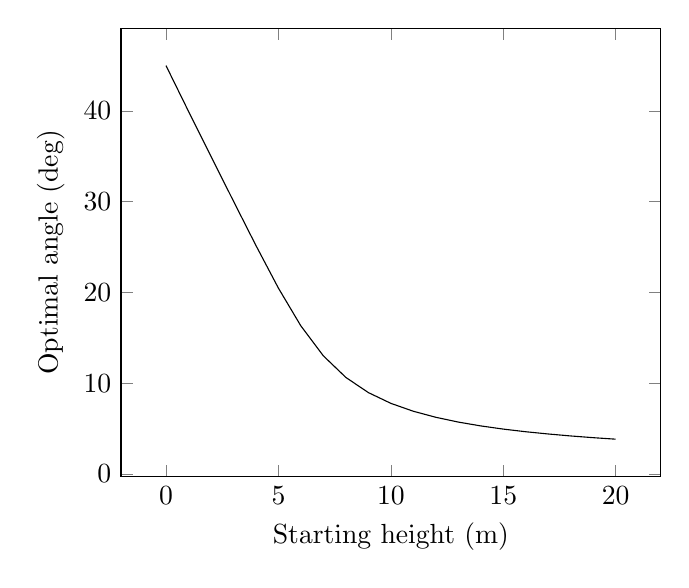
\begin{tikzpicture}
		\begin{axis}[ 
		xlabel=Starting height (m),
		ylabel=Optimal angle (deg)
		] 
		\addplot[solid] coordinates {(0, 44.9944) (1, 39.9581) (2, 34.9963) (3, 30.0631) (4, 25.1758) (5, 20.4775) (6, 16.3121) (7, 13.0176) (8, 10.6398) (9, 8.9725) (10, 7.7865) (11, 6.9156) (12, 6.2510) (13, 5.7238) (14, 5.2999) (15, 4.9504) (16, 4.6581) (17, 4.4118) (18, 4.1941) (19, 4.0050) (20, 3.8388) };
		\end{axis}
		\end{tikzpicture}
	\end{center}
	\begin{center}
		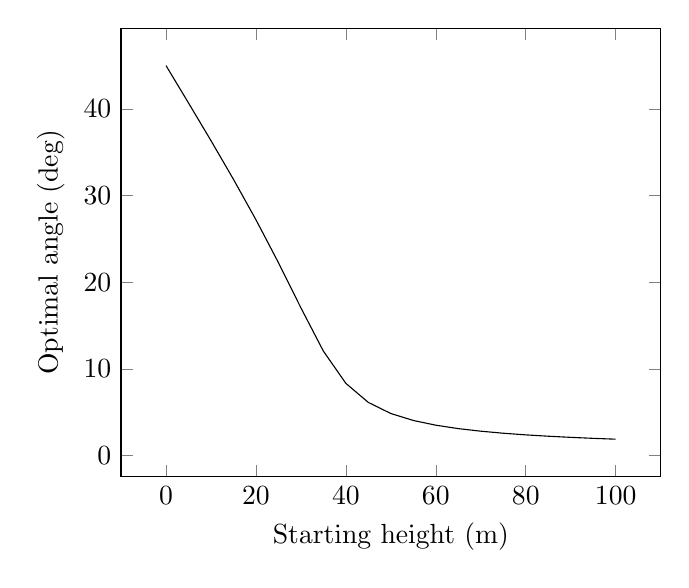
\begin{tikzpicture}
		\begin{axis}[ 
		xlabel=Starting height (m),
		ylabel=Optimal angle (deg)
		] 
		\addplot[solid] coordinates {(0, 44.9944) (5, 40.6857) (10, 36.3370) (15, 31.8736) (20, 27.2098) (25, 22.2594) (30, 17.0455) (35, 12.0493) (40, 8.3308) (45, 6.1306) (50, 4.8530) (55, 4.0508) (60, 3.5065) (65, 3.1112) (70, 2.8132) (75, 2.5783) (80, 2.3892) (85, 2.2345) (90, 2.1028) (95, 1.9882) (100, 1.8908) };
		\end{axis}
		\end{tikzpicture}
	\end{center}
	These graph both follow the same pattern that the distance gained from aiming upwards shrinks as the starting height increases. This is because the travel time cannot be changed all that much when the starting height already contributes so much to the distance.
	\\~\\
	The full code is available at GitHub\cite{code} and mostly contained in \texttt{math.js}. Algorithm \ref{alg:optimalAngle} can be found in the function \texttt{bestAngleFromStartingHeight()}.
	\section{Computational approach to air resistance}\label{seq:numericalAirRes}
	\subsection{Change at every time interval}
	At every time interval $\Delta\,t$ we can apply a force on our object in an angle opposite to $\beta$ proportional to our velocity $v$. While this does not give us a equation to work with we can use Euler's method to get a numerical approximation.
	
	Let $F_D$ be the force in the opposite direction of that which our object is traveling. At a time interval $\Delta t$ we will add a drag velocity $v_{drag}$ to our total velocity vector $v$.
	\begin{align}\nonumber
		\vec{v}_{new} = \vec{v}_{old} + \vec{v}_{drag}
	\end{align}
	In order to extrapolate $\vec{v}_{drag}$ from $F_D$ we need to consider our objects mass which we will denote $m$. This is due to 
	\begin{align}\nonumber
		\vec{F}=m\vec{a} = m\frac{\Delta\,\vec{v}}{\Delta\,t}\implies \Delta \vec{v} = \frac{\vec{F} \cdot \Delta\,t}{m} = \vec{v}_{drag}
	\end{align}
	This means is that the air resistance is inversely proportional the object's mass. While this might seem counterintuitive at first it is important to remember that a system with a higher mass means that the total energy of the system goes up. It is therefore only logical that our object travels further with higher mass; there is nowhere else for the extra energy to go. One can also consider conservation of momentum in terms of the air mass.
	\\~\\
	$\vec{F}_D$ is given by the quadratic drag equation
	\begin{align}\nonumber
		\vec{F}_D &= -\frac12\rho\,A\,C_D\,|v|^2\hat{v} \implies\\\nonumber
		\vec{v}_{drag} &= \begin{bmatrix}
			-0.5\,\rho\,A\,C_D\,v\,v_x\,m^{-1}\,\Delta\,t\\
			-0.5\,\rho\,A\,C_D\,v\,v_y\,m^{-1}\,\Delta\,t
		\end{bmatrix}
	\end{align}
	where $\rho$ is the air density, $A$ is the frontal area of our projectile, $m$ is the mass of the object and $C_D$ is the coefficient of drag which depends on the shape of our projectile. As $\Delta \rightarrow 0$ our calculations will be more computationally intensive but have greater accuracy.
	\subsection{Algorithm}
	We want a way to numerically apply a force to an object at every time interval and keep track of its velocity and position. The algorithm used can be summarized as the following.
	\begin{algorithm}[H]
		\caption{Algorithm for plotting projectile parabola with air resistance}
		\label{alg:airResistance}
		\begin{algorithmic}
			\Procedure{Air resistance array}{$v_0 ,\theta, \rho, C_D, m, y_0$}
			\State $g \gets $ $9.82$
			\State $x \gets 0$
			\State $y \gets y_0$
			\State $v_x \gets \cos\theta \cdot v_0$
			\State $v_y \gets \sin\theta \cdot v_0$
			\State $\Delta \, t \gets 0.001$;
			\State result $\gets$ [ ]
			\State
			\While {($y > 0$)}
			\State $v \gets \sqrt{v_x^2 + v_y^2}$
			\State $v_x \gets v_x - 0.5\cdot\rho\cdot C_D\cdot v\cdot v_x \cdot m^{-1}\cdot\Delta\,t$
			\State $v_y \gets v_y - 0.5\cdot\rho\cdot C_D\cdot v\cdot v_y \cdot m^{-1}\cdot\Delta\,t$
			\State
			\State $v_y \gets v_y -g \cdot \Delta \, t$
			\State
			\State $x \gets x + v_x \cdot \Delta\,t$
			\State $y \gets y + v_y \cdot \Delta\,t$
			\State
			\State result $\gets$ result $+$ ($x$, $y$)
			\EndWhile
			\State
			\State return result
			\EndProcedure
			
		\end{algorithmic}
	\end{algorithm}
	Using the above algorithm with initial data $v_0 =10,m/s$, $\theta = \ang{45} = \frac{\pi}{4}$, $\rho = 1.225\, kg/m^3$, $A = 1\,m^2$, $m = 1\,kg$, $y_0 = 0\,m$ and $C_D = 0.47$ yields the following result. The solid plot is with air resistance and the dashed plot is in a vacuum with the same $v_0$, $y_0$ and $\theta$.
	\begin{center}
		\begin{tikzpicture}
		\begin{axis}[ 
		xlabel=x (m),
		ylabel=y (m)
		] 
		\addplot[solid] coordinates {(0.0000, 0.0000) (0.2674, 0.2597) (0.5092, 0.4794) (0.7305, 0.6654) (0.9349, 0.8222) (1.1255, 0.9531) (1.3043, 1.0606) (1.4732, 1.1469) (1.6335, 1.2135) (1.7862, 1.2616) (1.9323, 1.2922) (2.0724, 1.3061) (2.2071, 1.3041) (2.3367, 1.2868) (2.4615, 1.2546) (2.5818, 1.2082) (2.6977, 1.1481) (2.8093, 1.0747) (2.9166, 0.9888) (3.0197, 0.8909) (3.1185, 0.7815) (3.2132, 0.6614) (3.3037, 0.5312) (3.3902, 0.3916) (3.4725, 0.2432) (3.5509, 0.0866) (3.5923, -0.0028) };
		
		\addplot[solid, dashed] coordinates {(0.0000, 0.0000) (0.2828, 0.2748) (0.5657, 0.5339) (0.8485, 0.7772) (1.1314, 1.0049) (1.4142, 1.2168) (1.6971, 1.4131) (1.9799, 1.5936) (2.2627, 1.7584) (2.5456, 1.9075) (2.8284, 2.0409) (3.1113, 2.1585) (3.3941, 2.2605) (3.6770, 2.3467) (3.9598, 2.4173) (4.2426, 2.4721) (4.5255, 2.5112) (4.8083, 2.5346) (5.0912, 2.5423) (5.3740, 2.5343) (5.6569, 2.5105) (5.9397, 2.4711) (6.2225, 2.4159) (6.5054, 2.3450) (6.7882, 2.2585) (7.0711, 2.1562) (7.3539, 2.0381) (7.6368, 1.9044) (7.9196, 1.7550) (8.2024, 1.5898) (8.4853, 1.4090) (8.7681, 1.2124) (9.0510, 1.0001) (9.3338, 0.7721) (9.6167, 0.5284) (9.8995, 0.2690) (10.1823, -0.0061) };
		
		\end{axis}
		\end{tikzpicture}
	\end{center}
	The full code is available at GitHub\cite{code} and mostly contained in \texttt{math.js}. Algorithm \ref{alg:airResistance} can be found in the functions \texttt{getAirResistanceData()} and \texttt{getAirResistance()}.
	\section{Analytical solution to one-dimensional air resistance}\label{seq:oneDim}
	\subsection{Derivation}\label{seq:oneDimIntro}
	Consider the simplest case of air resistance; the one-dimensional falling object. Our object does not travel in a parabola and we have previously described this motion as $y(t) = -\frac12gt^2+y_0$. Knowing the air resistance at any time $t$ we can construct a differential equation describing the motion of our object which is as follows
	\begin{align}\label{eq:oneDimAirResDiffEq}
		y''(t) = k\,y'(t)^2 - g \comma k = \frac{\frac12\rho\,A\,C_D}{m}\\\nonumber
		y(0) = y_0 \comma y'(0) = 0
	\end{align}
	\subsubsection{Position as a function of time}\label{seq:oneDimYt}
	We rewrite equation \eqref{eq:oneDimAirResDiffEq} with $v = y'$ and first solve for $v$. We can then determine $y$ as it is the antiderivative of $v$.
	\begin{align}\nonumber
		v'(t) = k\,v^2 - g &\implies \frac{v'}{k\, v^2 - g} = 1 \implies\\\label{eq:oneDimAirResGSolve}
		\int \frac{v'}{k\, v^2 - g}\,dt &= \int 1 \,dt = t + C := G
	\end{align}
	$C$ is a constant of integration which is added to $t$ at all times. Let $T = t + C \comma v' = \frac{dv}{dt}$. $G$ can now be written as the following in order to concentrate the unknowns
	\begin{align}\nonumber
		G=\int \frac{1}{k\, v^2-g}\,dv &= \int -\frac{1}{g(1-\frac{k\,v^2}{g})}\,dv \\\nonumber
		&= \int \frac{-1}{g} \frac{1}{1-\frac{k\,v^2}{g}}\,dv
	\end{align}
	To compress $G$ further we let $s^2 = \frac{k}{g}\,v^2 \implies s = \sqrt{\frac{k}{g}}\,v \implies \frac{ds}{dv} = \sqrt{\frac{k}{g}} \implies dv = \sqrt{\frac{g}{k}}\,ds$. We can now plug the alternative $dv$ and the new $s^2$ into $G$ to get rid of $\frac{k}{g}\,v^2$.
	\begin{align}\nonumber
		G = \int \Big(\frac{-1}{g} \, \frac{1}{1-s^2}\Big)\sqrt{\frac{g}{k}}\,ds &= \frac{-1}{\sqrt{gk}}\, \int \frac{1}{1-s^2}\,ds\\\nonumber
		&= \frac{-\tanh^{-1}(s)}{\sqrt{gk}}
	\end{align}
	Substituting back $s=\sqrt{\frac{k}{g}}\,v$ and recalling that $G = T$ we can  solve for $v$
	\begin{align}\nonumber
		G &= \frac{-\tanh^{-1}\big(\sqrt{\frac{k}{g}}\,v\big)}{\sqrt{gk}} = T \implies\\\nonumber
		\tanh^{-1}\Big(\sqrt{\frac{k}{g}}\,v\Big) &= -\sqrt{gk}\,T\implies\\\nonumber
		\sqrt{\frac{k}{g}}\,v &= \tanh(-\sqrt{gk}\,T) \implies \\\label{eq:oneDimAirResVT}
		v &= -\sqrt{\frac{g}{k}}\,\tanh(\sqrt{gk}\,T)
	\end{align}
	We let $C = 0$ since $v(0) = 0$ meaning $T = t$. We can now find $y$ as it is the antiderivative of $v$.
	\begin{align}\nonumber
		y = \int v\,dt = -\sqrt{\frac{g}{k}}\,\int \tanh(\sqrt{gk}\,t)\,dt
	\end{align}
	For simplicity; let $H = \int \tanh(\sqrt{gk}\,t)\,dt, c = \sqrt{gk}, s = c\,t \implies \frac{ds}{dt} = c \implies dt = \frac{ds}{c}$. The integral is now trivial and we can substitute back $s$ after evaluating it.
	\begin{align}\nonumber
		H = \int \tanh(s)\, \frac{ds}{c} &= \frac{1}{c} \ln(\cosh(s)) + y_0\\\nonumber
		&= \frac{\ln(\cosh(c\,T))}{c}+y_0
	\end{align}
	Substituting back $c$ and $H$ into $y$ we obtain our final expression.
	\begin{align}\nonumber
		y(t) &= -\sqrt{\frac{g}{k}}\,\frac{\ln(\cosh(\sqrt{gk}\,t))}{\sqrt{gk}} + y_0\\\label{eq:oneDimAirRes}
		&= \frac{-\ln(\cosh(\sqrt{gk}\,t))}{k} + y_0
	\end{align}
	\subsubsection{Determining the duration of the fall}
	In order to determine the duration of the fall we need to solve $y(t) = 0$ for $t$. This can be done from $y(t)$ alone without using any special methods.
	\begin{align}\nonumber
		y(t_{max}) &= \frac{-\ln(\cosh(\sqrt{gk}\,t_{max}))}{k} + y_0 = 0 \implies\\\nonumber
		y_0 &= \frac{\ln(\cosh(\sqrt{gk}\,t_{max}))}{k} \implies\\\nonumber
		y_0\,k &= \ln(\cosh(\sqrt{gk}\,t_{max})) \implies\\\nonumber
		\exp(y_0\,k) &= \cosh(\sqrt{gk}\,t_{max}) \implies\\\nonumber
		\sqrt{gk}\,t_{max} &= \cosh^{-1}(\exp(y_0\,k)) \implies\\\label{eq:oneDimAirResTMax}
		t_{max} &= \frac{\cosh^{-1}(\exp(y_0\,k))}{\sqrt{gk}}
	\end{align}
	\subsubsection{Terminal velocity}
	The terminal velocity of an object is the velocity at which it is no longer accelerating during a free fall because the air resistance is the same as the gravitational acceleration. We obtain this velocity by solving equation \eqref{eq:oneDimAirResDiffEq} for $y''(t) = 0$.
	\begin{align}\label{eq:oneDimAirResTerminalVel}
		k\,v_{term}^2 = g \implies v_{term} = \sqrt{\frac{g}{k}}
	\end{align}
	\subsection{Plots}\label{seq:airResPlots}
	We can analyse our function by plotting it and looking at its properties as well as compare it to a vacuum plot. All solid plots are generated with air resistance and dashed plots without.
	\\~\\
	The code for these plots can be found at GitHub\cite{code} and is contained in \texttt{freefall.html}.
	\subsubsection{Examples}
	This first image uses $k = 0.432$ which is derived from the following values roughly matching those of a beach ball.
	\begin{align}
		\begin{cases}\nonumber
			C_D &= 0.47 \\
			m &= 0.2\,kg\\
			y_0 &= 4\,m\\
			v_0 &= 0\,m/s\\
			\rho &= 1.225\,kg/m^3\\
			A &= 0.3\,m^2
		\end{cases}
	\end{align}
	\begin{center}
		\begin{tikzpicture}
		\begin{axis}[ xlabel=t (s), ylabel=y (m)]
		
		\addplot[solid] coordinates {(0.000, 4.000) (0.010, 4.000) (0.020, 3.998) (0.030, 3.996) (0.040, 3.992) (0.050, 3.988) (0.060, 3.982) (0.070, 3.976) (0.080, 3.969) (0.090, 3.960) (0.100, 3.951) (0.110, 3.941) (0.120, 3.930) (0.130, 3.918) (0.140, 3.905) (0.150, 3.891) (0.160, 3.877) (0.170, 3.861) (0.180, 3.844) (0.190, 3.827) (0.200, 3.809) (0.210, 3.790) (0.220, 3.770) (0.230, 3.749) (0.240, 3.728) (0.250, 3.706) (0.260, 3.683) (0.270, 3.659) (0.280, 3.635) (0.290, 3.610) (0.300, 3.584) (0.310, 3.557) (0.320, 3.530) (0.330, 3.502) (0.340, 3.474) (0.350, 3.444) (0.360, 3.415) (0.370, 3.384) (0.380, 3.353) (0.390, 3.322) (0.400, 3.290) (0.410, 3.257) (0.420, 3.224) (0.430, 3.191) (0.440, 3.157) (0.450, 3.122) (0.460, 3.087) (0.470, 3.052) (0.480, 3.016) (0.490, 2.980) (0.500, 2.943) (0.510, 2.906) (0.520, 2.868) (0.530, 2.830) (0.540, 2.792) (0.550, 2.754) (0.560, 2.715) (0.570, 2.676) (0.580, 2.636) (0.590, 2.596) (0.600, 2.556) (0.610, 2.516) (0.620, 2.475) (0.630, 2.434) (0.640, 2.393) (0.650, 2.352) (0.660, 2.310) (0.670, 2.268) (0.680, 2.226) (0.690, 2.184) (0.700, 2.141) (0.710, 2.098) (0.720, 2.055) (0.730, 2.012) (0.740, 1.969) (0.750, 1.926) (0.760, 1.882) (0.770, 1.838) (0.780, 1.794) (0.790, 1.750) (0.800, 1.706) (0.810, 1.662) (0.820, 1.617) (0.830, 1.573) (0.840, 1.528) (0.850, 1.483) (0.860, 1.438) (0.870, 1.393) (0.880, 1.348) (0.890, 1.303) (0.900, 1.257) (0.910, 1.212) (0.920, 1.166) (0.930, 1.121) (0.940, 1.075) (0.950, 1.029) (0.960, 0.984) (0.970, 0.938) (0.980, 0.892) (0.990, 0.846) (1.000, 0.799) (1.010, 0.753) (1.020, 0.707) (1.030, 0.661) (1.040, 0.614) (1.050, 0.568) (1.060, 0.521) (1.070, 0.475) (1.080, 0.428) (1.090, 0.382) (1.100, 0.335) (1.110, 0.289) (1.120, 0.242) (1.130, 0.195) (1.140, 0.148) (1.150, 0.101) (1.160, 0.055) (1.170, 0.008) (1.180, -0.039) };
		
		\addplot[solid, dashed] coordinates {(0.000, 4.000) (0.010, 4.000) (0.020, 3.998) (0.030, 3.996) (0.040, 3.992) (0.050, 3.988) (0.060, 3.982) (0.070, 3.976) (0.080, 3.969) (0.090, 3.960) (0.100, 3.951) (0.110, 3.941) (0.120, 3.929) (0.130, 3.917) (0.140, 3.904) (0.150, 3.890) (0.160, 3.874) (0.170, 3.858) (0.180, 3.841) (0.190, 3.823) (0.200, 3.804) (0.210, 3.783) (0.220, 3.762) (0.230, 3.740) (0.240, 3.717) (0.250, 3.693) (0.260, 3.668) (0.270, 3.642) (0.280, 3.615) (0.290, 3.587) (0.300, 3.558) (0.310, 3.528) (0.320, 3.497) (0.330, 3.465) (0.340, 3.432) (0.350, 3.399) (0.360, 3.364) (0.370, 3.328) (0.380, 3.291) (0.390, 3.253) (0.400, 3.214) (0.410, 3.175) (0.420, 3.134) (0.430, 3.092) (0.440, 3.049) (0.450, 3.006) (0.460, 2.961) (0.470, 2.915) (0.480, 2.869) (0.490, 2.821) (0.500, 2.772) (0.510, 2.723) (0.520, 2.672) (0.530, 2.621) (0.540, 2.568) (0.550, 2.515) (0.560, 2.460) (0.570, 2.405) (0.580, 2.348) (0.590, 2.291) (0.600, 2.232) (0.610, 2.173) (0.620, 2.113) (0.630, 2.051) (0.640, 1.989) (0.650, 1.926) (0.660, 1.861) (0.670, 1.796) (0.680, 1.730) (0.690, 1.662) (0.700, 1.594) (0.710, 1.525) (0.720, 1.455) (0.730, 1.383) (0.740, 1.311) (0.750, 1.238) (0.760, 1.164) (0.770, 1.089) (0.780, 1.013) (0.790, 0.936) (0.800, 0.858) (0.810, 0.779) (0.820, 0.699) (0.830, 0.618) (0.840, 0.536) (0.850, 0.453) (0.860, 0.369) (0.870, 0.284) (0.880, 0.198) (0.890, 0.111) (0.900, 0.023) (0.910, -0.066) };
		\end{axis}
		\end{tikzpicture}
	\end{center}
	The slow start with a negative second derivative matches our intuition and at roughly $t = 0.8\,s$ the first derivative appears to approach zero. This should be due to the object reaching its terminal velocity which we can calculate using equation \eqref{eq:oneDimAirResTerminalVel}.
	\begin{align}\nonumber
		v_{max} = \sqrt{\frac{g}{k}} = \sqrt{\frac{9.82}{0.432}} = 4.77\,m/s
	\end{align}
	We can approximate the derivative at $t=0.8$ as $\frac{\Delta y}{\Delta t} \approx 4.4 \approx v_{max}$. Equation \eqref{eq:oneDimAirResTMax} also predicts a $t_{max}$ which can be tested.
	\begin{align}\nonumber
		t_{max} = \frac{\cosh^{-1}(\exp(y_0\,k))}{\sqrt{gk}} = \frac{\cosh^{-1}(\exp(1.728))}{\sqrt{4.424224}} \approx 1.17\,s
	\end{align}
	The plot reports $t_{max} \approx 1.17\,s$. Comparing this to a vacuum solution we can use equation \eqref{eq:tMaxFromHeight} which gives
	\begin{align}\nonumber
		t_{max} &= \frac{v_0\sin\theta}{g}+\frac{\sqrt{v_{0}^2\sin^2\theta+2g\,y_0}}{g}\\\nonumber
		&= \frac{\sqrt{2\,g\,y_0}}{g} = \frac{\sqrt{78.56}}{9.82} \approx 0.90\,s
	\end{align}
	This is a major discrepancy which adds credit to the accuracy of equation \eqref{eq:oneDimAirResTMax}.
	
	We can plot another $y(t)$ where $k$ is much smaller which should result in our object not reaching its terminal velocity in such short time. The following measurements are from a small steel ball with $k = 0.00313$.
	\begin{align}\nonumber
		\begin{cases}\nonumber
			C_D &= 0.47 \\
			m &= 0.022\,kg\\
			y_0 &= 3\,m\\
			v_0 &= 0\,m/s\\
			\rho &= 1.225\,kg/m^3\\
			A &= 0.00023916\,m^2
		\end{cases}
	\end{align}
	\begin{center}
		\begin{tikzpicture}
		\begin{axis}[ xlabel=t (s), ylabel=y (m)]
		\addplot[solid] coordinates {(0.000, 3.000) (0.010, 3.000) (0.020, 2.998) (0.030, 2.996) (0.040, 2.992) (0.050, 2.988) (0.060, 2.982) (0.070, 2.976) (0.080, 2.969) (0.090, 2.960) (0.100, 2.951) (0.110, 2.941) (0.120, 2.929) (0.130, 2.917) (0.140, 2.904) (0.150, 2.890) (0.160, 2.874) (0.170, 2.858) (0.180, 2.841) (0.190, 2.823) (0.200, 2.804) (0.210, 2.784) (0.220, 2.762) (0.230, 2.740) (0.240, 2.717) (0.250, 2.693) (0.260, 2.668) (0.270, 2.642) (0.280, 2.615) (0.290, 2.587) (0.300, 2.558) (0.310, 2.528) (0.320, 2.497) (0.330, 2.466) (0.340, 2.433) (0.350, 2.399) (0.360, 2.364) (0.370, 2.328) (0.380, 2.292) (0.390, 2.254) (0.400, 2.215) (0.410, 2.175) (0.420, 2.135) (0.430, 2.093) (0.440, 2.050) (0.450, 2.007) (0.460, 1.962) (0.470, 1.917) (0.480, 1.870) (0.490, 1.823) (0.500, 1.774) (0.510, 1.725) (0.520, 1.674) (0.530, 1.623) (0.540, 1.570) (0.550, 1.517) (0.560, 1.463) (0.570, 1.407) (0.580, 1.351) (0.590, 1.294) (0.600, 1.236) (0.610, 1.176) (0.620, 1.116) (0.630, 1.055) (0.640, 0.993) (0.650, 0.930) (0.660, 0.866) (0.670, 0.801) (0.680, 0.735) (0.690, 0.668) (0.700, 0.600) (0.710, 0.531) (0.720, 0.461) (0.730, 0.391) (0.740, 0.319) (0.750, 0.246) (0.760, 0.172) (0.770, 0.098) (0.780, 0.022) (0.790, -0.055) };
		
		\addplot[solid, dashed] coordinates {(0.000, 3.000) (0.010, 3.000) (0.020, 2.998) (0.030, 2.996) (0.040, 2.992) (0.050, 2.988) (0.060, 2.982) (0.070, 2.976) (0.080, 2.969) (0.090, 2.960) (0.100, 2.951) (0.110, 2.941) (0.120, 2.929) (0.130, 2.917) (0.140, 2.904) (0.150, 2.890) (0.160, 2.874) (0.170, 2.858) (0.180, 2.841) (0.190, 2.823) (0.200, 2.804) (0.210, 2.783) (0.220, 2.762) (0.230, 2.740) (0.240, 2.717) (0.250, 2.693) (0.260, 2.668) (0.270, 2.642) (0.280, 2.615) (0.290, 2.587) (0.300, 2.558) (0.310, 2.528) (0.320, 2.497) (0.330, 2.465) (0.340, 2.432) (0.350, 2.399) (0.360, 2.364) (0.370, 2.328) (0.380, 2.291) (0.390, 2.253) (0.400, 2.214) (0.410, 2.175) (0.420, 2.134) (0.430, 2.092) (0.440, 2.049) (0.450, 2.006) (0.460, 1.961) (0.470, 1.915) (0.480, 1.869) (0.490, 1.821) (0.500, 1.772) (0.510, 1.723) (0.520, 1.672) (0.530, 1.621) (0.540, 1.568) (0.550, 1.515) (0.560, 1.460) (0.570, 1.405) (0.580, 1.348) (0.590, 1.291) (0.600, 1.232) (0.610, 1.173) (0.620, 1.113) (0.630, 1.051) (0.640, 0.989) (0.650, 0.926) (0.660, 0.861) (0.670, 0.796) (0.680, 0.730) (0.690, 0.662) (0.700, 0.594) (0.710, 0.525) (0.720, 0.455) (0.730, 0.383) (0.740, 0.311) (0.750, 0.238) (0.760, 0.164) (0.770, 0.089) (0.780, 0.013) (0.790, -0.064) };
		
		\end{axis}
		\end{tikzpicture}
	\end{center}
	Here equation \eqref{eq:tMaxFromHeight} gives $t_{max} = 0.7817\,s$, equation \eqref{eq:oneDimAirResTMax} gives $t_{max} = 0.7830\,s$ and the plot gives $t_{max} = 0.7829\,s$. Air resistance plays almost no part here and the dashed plot is nearly indistinguishable from the solid one.
	\subsubsection{Analysis}
	As the second example showed it is mainly the terminal velocity which causes the lower overall velocity of a falling object with air resistance compared to one in a vacuum. This is a logical consequence of the fact that the mass of the air displaced by a falling body generally is small compared to that of the falling object.
	\\~\\
	As shown in the second example for an object with a small $k$ value air resistance is negligible and the methods detailed in section \ref{seq:properties} and \ref{seq:resultValues} provide an accurate description of reality.
	\section{Analytical approximations to two-dimensional air resistance}
	\subsection{Introduction}
	We wish to extend the solutions developed in section \ref{seq:oneDim} to work in two dimensions. We let $u = v_x$ and $w = v_y$ in order to make it easier to separate them. In general we can write the drag equations as
	\begin{align}\nonumber
		\vec{F} = m\vec{a} &= -mkv^2\hat{v} - mg\hat{\jmath} = -mkv\vec{v}-mg\hat{\jmath} \implies\\\nonumber
		\vec{a} &= -kv\vec{v}-g\hat{\jmath}\comma \vec{v} = \begin{bmatrix}
			-kv\cos\alpha\,\vec{v}\\
			-kv\sin\alpha\,\vec{v}-g\\
		\end{bmatrix}\implies  \\\nonumber
		u' &= -kvu \comma w' = -kvw-g\,\,\,\,\,
	\end{align}
	where $v = ||\vec{v}|| = \sqrt{u^2+w^2}$ and $\alpha$ is the angle the object is traveling in at an arbitrary time. This means that $u$ is dependent on $w$ and the other way around. In order to work around this we need to make approximations regarding the relationship between $u$ and $w$ to eliminate $v$ from their differential equations of motion. The following three options are the ways to express $v$ in terms of only one variable.
	\begin{align}\nonumber
		v \approx
		\begin{cases}
			u			&if\,\,\, u \gg w\\
			w			&if\,\,\, w \gg w\\
			\sqrt{2}u	&if\,\,\, u \approx w\\
		\end{cases}\\\nonumber
	\end{align}
	We treat these as three separate cases and label them as LAT, HAT and SAT for Low Angle Trajectory, High Angle Trajectory and Split Angle Trajectory respectively.
	\subsection{Low Angle Trajectory approximation}\label{seq:lat}
	\subsubsection{Differential equations of motion}
	With a low angle trajectory we assume $v \approx u$ since $u \gg w$. Subsequently our differential equations of motion become the following.
	\begin{align}\label{eq:twoDimEMOLATU}
		u' &= -ku^2\comma u(0) = u_0\\\label{eq:twoDimEMOLATW}
		w' &= -kwu-g\comma w(0) = w_0
	\end{align}
	\subsubsection{Velocity}
	We begin by solving equation \eqref{eq:twoDimEMOLATU} for $u$.
	\begin{align}\nonumber
	u' &= -k\,u^2 \implies \int \frac{\frac{du}{dt}}{u^2}\,dt = \int -k\,dt = -kt + 
	c_1\\\nonumber
	&= \int \frac{1}{u^2}\,du = \frac{-1}{u} +c_2 \implies \frac{1}{u} = kt - C \implies \\\nonumber
	u &= \frac{1}{kt-C} \comma u(0) = u_0 \implies u_0 = \frac{-1}{C} \implies\\\label{eq:twoDimU}
	C &= \frac{-1}{u_0} \implies u = \frac{u_0}{u_0kt+1}
	\end{align}
	We can now plus $u$ from equation \eqref{eq:twoDimU} into equation \eqref{eq:twoDimEMOLATW} and solve for $w$.
	\begin{align}\nonumber
		w' = -kuw-g = \frac{-ku_0w}{u_0kt+1}-g
	\end{align}
	Let $a = ku_0$. We can now solve the differential equation for $w$. Let $\mu = at+1 \implies \frac{d\mu}{dt} = a$.
	\begin{align}\nonumber
		\frac{dw}{dt} = \frac{-aw}{at+1}-g \implies \frac{dw}{dt} + \frac{aw}{\mu} &= -g \implies\\\nonumber
		\frac{dw}{dt}\,\mu + aw &= -g\,\mu \\\label{eq:twoDimWProd}
		=\frac{dw}{dt}\,\mu + \frac{d\mu}{dt}\,w &= -g\,\mu\\\nonumber
	\end{align}
	From the product rule we know that $\frac{d}{dt}(f\,g) = \frac{df}{dt}\,g+\frac{dg}{dt}\,f$. Applying this reversely to equation \eqref{eq:twoDimWProd} we get
	\begin{align}\nonumber
		\frac{d}{dt}(w\,\mu) &= -g\,\mu\implies\int\frac{d}{dt}\,(w\,\mu)\,dt\\\nonumber
		= -g\,\int \mu\,dt = w\,\mu+c_1 &= -g(\frac{at^2}{2}+t)+c_2\implies\\\nonumber
		w = \frac{-g(\frac{at^2}{2}+t)+C}{\mu} &= \frac{-gat^2}{2\mu}-\frac{gt}{\mu}+\frac{C}{\mu}
	\end{align}
	Solving for the initial condition $w(0) = w_0$ we obtain our final expression for $w$.
	\begin{align}\nonumber
		w(0) &= \frac{C}{a\cdot 0+1} = w_0 \implies C = w_0 \implies\\\nonumber
		w &= \frac{-gat^2}{2\mu}-\frac{gt}{\mu}+\frac{w_0}{\mu} = \frac{-gat^2-2gt+2w_0}{2\mu}\\\nonumber
		&= \frac{-g\frac{at^2}{2}-gt+w_0}{\mu} = \frac{-gt(\frac{at}{2}+1)+w_0}{at+1}
	\end{align}
	\subsubsection{Position}
	Now that we have obtained the velocity functions for $u$ and $w$ we can construct the functions $x(t)$ and $y(t)$ as their respective indefinite integrals. Let $x(0) = x_0$ and $y(0) = y_0$.
	\begin{align}\nonumber
		x = \int u\,dt = \int \frac{u_0}{u_0kt+1}\,dt = u_0\,\int\frac{1}{u_0kt+1}\,dt
	\end{align}
	Let $s = u_0kt+1 \implies \frac{ds}{dt} = u_0k \implies dt = \frac{ds}{u_0k}$.
	\begin{align}\nonumber
		x &= u_0\,\int\frac{1}{s}\,\frac{ds}{u_0k} = \frac{1}{k}\,\int\frac{1}{s}\,ds\\\nonumber
		&= \frac{\ln s}{k} + C = \frac{\ln(u_0kt+1)}{k} + x_0
	\end{align}
	We can solve for $y$ the same way but begin by writing $w$ as a sum of terms and determining its indefinite integral.
	\begin{align}\nonumber
		w &= \frac{-gt(\frac{at}{2}+1)+w_0}{at+1} = \frac{2aw_0+g}{2a(at+1)}-\frac{g}{2a}-\frac{gt}{2}\\\nonumber
		y &= \int w\,dt = \int \Big(\frac{2aw_0+g}{2a(at+1)}-\frac{g}{2a}-\frac{gt}{2}\Big)\,dt \\\nonumber
		&=\big(\frac{g}{2a}+w_0\big)\int\frac{1}{at+1}\,dt -\frac{g}{2a}\int 1\,dt -\frac{g}{2}\int t\,dt\\\nonumber
		&=\big(\frac{g}{2a}+w_0\big)\,\frac{1}{a}\ln(at+1) -\frac{gt}{2a}-\frac{gt^2}{4}+y_0
	\end{align}
	\subsubsection{Equations of motion}
	Having solved equation \eqref{eq:twoDimEMOLATU} and \eqref{eq:twoDimEMOLATW} we can write out all the equations of motion for LAT.
	\begin{align*}\nonumber
		u(t) &= \frac{u_0}{\mu}\\\nonumber
		w(t) &= \frac{-gt(\frac{at}{2}+1)+w_0}{\mu}\\\nonumber
		x(t) &= \frac{\ln(\mu)}{k} + x_0\\\nonumber
		y(t) &= \big(\frac{g}{2a}+w_0\big)\frac{1}{a}\ln(\mu) -\frac{gt}{2a}-\frac{gt^2}{4}+y_0\\\nonumber
		&\mathrm{where}\,\,\mu = at+1 \comma a = ku_0
	\end{align*}
	\subsection{High Angle Trajectory approximation}\label{seq:hat}
	With high angle trajectories we assume $v \approx w$ since $w \gg u$. We can now write our differential equations of motion as the following.
	\begin{align}\label{eq:twoDimEOMDIFFBASE}
		u' = -ku|w| \comma w' -k|w|w-g
	\end{align}
	In contrary to our LAT approximation in section \ref{seq:lat} we must now separate the cases where $\hat{w} = \hat{\jmath}, \hat{w} = -\hat{\jmath}$ because a negative $w$ should not lead to a positive $u'$. When $v$ was approximated as $u$ we assumed that $\hat{u} = \hat{\imath}$ because it is the only realistic scenario. Now that $v$ is approximated as $w$ we need to consider its direction before that context. In the end our equations of motions will consist of two separate $u$ and $w$.
	\subsubsection{Differential equations of motion}
	The following are all the differential equations of motion derived from equation \eqref{eq:twoDimEOMDIFFBASE} and separated by ascending and descending.
	\begin{align}\label{eq:twoDimEOMHATUP}
		u_{+}' &= -kuw_+ \comma u_+(0) = u_{+0}\\\label{eq:twoDimEOMHATWP}
		w_{+}' &= -kw^2 -g \comma w_+(0) = w_{+0}\\\label{eq:twoDimEOMHATUM}
		u_{-}' &= -kuw_- \comma u_-(0) = u_{-0}\\\label{eq:twoDimEOMHATWM}
		w_{-}' &=  kw^2 -g \comma w_-(0) = w_{-0}
	\end{align}
	\subsubsection{Ascending velocity}
	For the purpose of this section we will drop the "$+$" postfix. We begin by solving equation \eqref{eq:twoDimEOMHATWP} in order to be able to express equation \eqref{eq:twoDimEOMHATUP} as a function of one variable. This is the same as equation \eqref{eq:oneDimAirResGSolve} with the only difference being the sign of $k\,v^2$. It can be shown that using the same technique as that in section \ref{seq:oneDimYt} we can derive equation \eqref{eq:oneDimAirResVT} but with $\tan(\sqrt{gk}\,T)$ instead of $\tanh(\sqrt{gk}\,T)$. From here we can solve for our initial condition $w(0) = w_0$.
	\begin{align}\nonumber
		w &= -\sqrt{\frac{g}{k}}\,\tan(\sqrt{gk}\,(t + C))\\\nonumber
		w_o &= -\sqrt{\frac{g}{k}}\,\tan(\sqrt{gk}\,C) \implies\\\nonumber
		C &= \frac{-\arctan\big(w_0\sqrt{\frac{k}{g}}\big)}{\sqrt{gk}} \implies\\\label{eq:twoDimEOMHATWPSOLVE}
		w &= \sqrt{\frac{g}{k}}\,\tan\big(\arctan\big(w_0\sqrt{\frac{k}{g}}\big) - \sqrt{gk}\,t\big)
	\end{align}
	Having solved for $w$ we can now solve equation \eqref{eq:twoDimEOMHATUP} for $u$. To shorten equation \eqref{eq:twoDimEOMHATWPSOLVE} we let $\omega = \sqrt{gk} \comma \varphi = \arctan\big(w_0\sqrt{\frac{k}{g}}\big)$. We can compress the constants as $-k\sqrt{\frac{g}{k}} = -\omega$.
	\begin{align}\nonumber 
		u' &= -ukw = -u\omega\tan(\varphi-\omega\,t) \implies\\\nonumber
		\int\frac{\frac{du}{dt}}{u}\,dt &= \int-\omega\tan(\varphi-\omega t)\,dt = \\\nonumber
		\int\frac{1}{u}\,dt &= -\omega\int\tan(\varphi-\omega t)\, dt
	\end{align}
	Let $s = \varphi-\omega t \implies \frac{ds}{dt} = -\omega \implies dt =  \frac{ds}{-\omega}$.
	\begin{align}\nonumber
		\ln u + c_1 &= \frac{-\omega}{-\omega}\int\tan s\,ds = -\ln(\cos(s)) +c_2 \implies\\\nonumber
		u &= \exp(-\ln(\cos(s)) + C)\\\nonumber
		&= \big(\cos(\varphi - \omega t)\big)^{-1}\,e^C = \frac{e^C}{\cos(\varphi - \omega t)}\\\label{eq:twoDimEOMHATUPSOLVE}
		u_0 &= \frac{e^C}{\cos\varphi} \implies u = \frac{u_0\cos\varphi}{\cos(\varphi - \omega t)}
	\end{align}
	\subsubsection{Ascending position}
	For our ascending positions we determine the indefinite integrals of equation \eqref{eq:twoDimEOMHATUPSOLVE} and \eqref{eq:twoDimEOMHATWPSOLVE}. For both equations we let $s = \varphi - \omega t \implies \frac{ds}{dt} = -\omega \implies dt = \frac{ds}{-\omega}$. We begin by solving for $x$ with $x(0) = x_0$.
	\begin{align}\nonumber
		x &= \int u\,dt = \int \frac{u_0\cos\varphi}{\omega}\,dt\\\nonumber
		&= u_0\cos\varphi\int \frac{1}{\cos s}\,dt = \frac{u_0\cos\varphi}{-\omega}\int \sec s\,ds\\\nonumber
		&= \frac{u_0\cos\varphi}{-\omega}\,\Big\lbrack\ln(\tan s+\sec s) + C\Big\rbrack \implies\\\nonumber
		x_0 &= \frac{u_0\cos\varphi}{-\omega}\,\Big\lbrack\ln(\tan\varphi+\sec\varphi) + C\Big\rbrack \implies\\\nonumber
		C &= \frac{-x_0\omega}{u_0\cos\varphi}-\ln(\tan\varphi+\sec\varphi) \implies\\\label{eq:twoDimHATXFIN}
		x &= \frac{-u_0\cos\varphi}{\omega}\,\ln\Bigg\lbrack\frac{\tan(\varphi-\omega t)+\sec(\varphi-\omega t)}{\tan\varphi+\sec\varphi}\Bigg\rbrack +x_0
	\end{align}
	For $y$ the procedure is essentially the same.
	\begin{align}\nonumber
		y &= \int w \,dt = \int \sqrt{\frac{g}{k}} \tan(\varphi - \omega t)\,dt\\\nonumber
		&= \sqrt{\frac{g}{k}} \int \tan s \,dt = \frac{\sqrt{\frac{g}{k}}}{-\omega} \int \tan s\,ds\\\nonumber
		&=\frac{\sqrt{\frac{g}{k}}}{\sqrt{gk}} \ln(\cos s) + C = \frac{1}{k}\big(\ln(\cos(\varphi - \omega t)) + C\big)\\\nonumber
		y(0) &= y_0 \implies C = y_0k-\ln(\cos\varphi) \implies\\\label{eq:twoDimHATYFIN}
		y &= \frac{1}{k}\ln\Bigg\lbrack\frac{\cos(\varphi-\omega t)}{\cos\varphi}\Bigg\rbrack+y_0
	\end{align}
	\subsubsection{Descending velocity}\label{seq:twoDimDesVel}
	For our initial conditions want the final $x(t)$ and $y(t)$ to be continuous at all times $t$. Therefore the following initial conditions must hold.
	\begin{align}\nonumber
		u_{-}(0) &= u_{+}(t_{turn})\\\nonumber
		w_{-}(0) &= w_{+}(t_{turn})
	\end{align}
	Here $t_{turn}$ is defined as $w_+(t_{turn}) = \omega\,t_{turn}-\varphi = 0$ i.e. $t_{turn} = \frac{\varphi}{\omega}$. We can introduce the variable $\tau$ and define it as $\tau = t-t_{turn}$ meaning when $t = t_{turn} \comma \tau = 0$ and let $u_{-}$ and $w_{-}$ be functions of $\tau$. We begin by solving $u_+(t_{turn})$ and $w_+(t_{turn})$ for our initial conditions.
	\begin{align}\nonumber
		u_+(t_{turn}) &= \frac{u_0\cos\varphi}{\cos(\varphi-\varphi)} = u_0\cos\varphi\\\nonumber
		w_+(t_{turn}) &= \sqrt{\frac{g}{k}}\tan(\varphi-\varphi) = 0
	\end{align}
	Having established our initial conditions we can drop the $-$ postfix. Analysing equation \eqref{eq:twoDimEOMHATWM} we can see that it is the same as equation \eqref{eq:oneDimAirResDiffEq}. We can solve it the same way and find the following expression for $w$.
	\begin{align}\label{eq:twoDimHATMWFIN}
		w =-\sqrt{\frac{g}{k}}\,\tanh(\omega\,\tau)
	\end{align}
	Using the above expression for $w$ we can solve equation \eqref{eq:twoDimEOMHATUM} for $u$ with the initial condition $u(0) = u_0\cos\varphi$ where $u_0$ is the $x$ component of the initial launch velocity.
	\begin{align}\nonumber
		u' &= -k\sqrt{\frac{g}{k}}\tanh(\omega \tau)\,u = -u\,\omega\tanh(\omega\tau) \implies\\\nonumber
		\int \frac{\frac{du}{dt}}{u}\,dt &= \int -\omega\tanh(\omega\tau)\,dt \implies\\\nonumber
		\ln u &= \frac{\omega}{\omega}\ln(\cosh(\omega\tau)) + c_1 \implies u = e^{c_1}\sech(\omega\tau)\\\label{eq:twoDimHATMUFIN}
		u(0) &= u_0\cos\varphi \implies u = u_0\cos\varphi\sech(\omega\tau)
	\end{align}
	\subsubsection{Descending position}
	We adopt the same conventions detailed in section \ref{seq:twoDimDesVel} regarding $\tau$. For our position functions we take the antiderivative of equation \eqref{eq:twoDimHATMWFIN} and equation \eqref{eq:twoDimHATMUFIN}. We want $x_{-}(0) = x_{+}(t_{turn})$ and $y_{-}(0) = y_{+}(t_{turn})$. To determine these initial conditions we plug $t = \frac{\varphi}{\omega}$ into equation \eqref{eq:twoDimHATXFIN} and equation \eqref{eq:twoDimHATYFIN}.
	\begin{align}\nonumber
		x_{+}(\frac{\varphi}{\omega}) &= \frac{-u_0\cos\varphi}{\omega}\,\ln\Bigg\lbrack\frac{\tan(\varphi-\varphi)+\sec(\varphi-\varphi)}{\tan\varphi+\sec\varphi}\Bigg\rbrack +x_0 \\\label{eq:twoDimHATDXTURN}
		&= \frac{-u_0\cos\varphi}{\omega}\,\ln\Bigg\lbrack\frac{1}{\tan\varphi+\sec\varphi}\Bigg\rbrack +x_0\\\nonumber
		y_{+}(\frac{\varphi}{\omega}) &= \frac{1}{k}\ln\Bigg\lbrack\frac{\cos(\varphi-\varphi)}{\cos\varphi}\Bigg\rbrack+y_0\\\label{eq:twoDimHATDYTURN}
		&= \frac{1}{k}\ln\Bigg\lbrack\frac{1}{\cos\varphi}\Bigg\rbrack+y_0
	\end{align}
	We can now drop the $-$ and $+$ postfixes and solve equation \eqref{eq:twoDimHATMUFIN} for $x$.
	\begin{align}\nonumber
		x &= \int u\,d\tau = \int u_0\cos\varphi\sech(\omega\tau)\,d\tau\\\nonumber
		&= u_0\cos\varphi\int\sech(\omega\tau)\,d\tau
	\end{align}
	We solve the indefinite integral separately since $u_0\cos\varphi$ doesn't depend on $\tau$. Let $F = \int\sech(\omega\tau)\,d\tau \comma \gamma = \omega\tau \implies \frac{d\gamma}{d\tau} = \omega \implies d\tau = \frac{d\gamma}{\omega}$.
	\begin{align}\nonumber
		F=\frac{1}{\omega}\int\sech\gamma\,d\gamma = \frac{1}{\omega}\int \frac{1}{\cosh\gamma} \,d\gamma = \frac{1}{\omega}\int \frac{\cosh\gamma}{\cosh^2\gamma} \,d\gamma
	\end{align}
	Using the trigonometric identity $\cosh^2x - \sinh^2x = 1$ we can rewrite $F$ as the following.
	\begin{align}\nonumber
		F = \frac{1}{\omega}\int \frac{\cosh\gamma}{\sinh^2\gamma+1} \,d\gamma
	\end{align}
	Let $s = \sinh\gamma \implies \frac{ds}{d\gamma} = \cosh\gamma \implies d\gamma = \frac{ds}{\cosh\gamma}$.
	\begin{align}\nonumber
		F &= \frac{1}{\omega}\int \frac{\cosh\gamma}{s^2+1} \,\frac{ds}{\cosh\gamma} = \frac{1}{\omega}\int \frac{1}{s^2+1} \,ds\\\nonumber
		&= \frac{\arctan s}{\omega} + c_1 = \frac{\arctan(\sinh(\omega\tau))}{\omega}+c_1 \implies\\\nonumber
		x &= \frac{u_0\cos\varphi\arctan(\sinh(\omega\tau))}{\omega} + C
	\end{align}
	Plugging our initial condition from equation \eqref{eq:twoDimHATDXTURN} we obtain our final expression for $x$.
	\begin{align}\nonumber
		x = \frac{u_0\cos\varphi}{\omega}\Bigg\lbrack \arctan(\sinh(\omega\tau)) - \ln\Big(\frac{1}{\tan\varphi+\sec\varphi}\Big)  \Bigg\rbrack+x_0
	\end{align}
	We can now solve for $y$ with the initial condition derived in equation \eqref{eq:twoDimHATDYTURN}. As for the general solution it was derived in section \ref{seq:oneDimYt} and determined in equation \eqref{eq:oneDimAirRes}. Plugging the initial condition we obtain the following expression for $y$.
	\begin{align}\nonumber
		y &= \frac{-\ln(\cosh(\sqrt{gk}\,\tau))}{k} + y_{+}(t_{turn})\\\nonumber
		&= \frac{1}{k}\ln\Big(\frac{1}{\cos\varphi\cosh(\omega\tau)}\Big) + y_0
	\end{align}
	\subsubsection{Equations of motion}
	We can now write out all the equations of motion for HAT.
	\begin{align*}\nonumber
		u_{+}(t) &= \frac{u_0\cos\varphi}{\cos(\varphi - \omega t)}\\\nonumber
		w_{+}(t) &= \sqrt{\frac{g}{k}}\,\tan(\varphi - \omega\,t)\\\nonumber
		x_{+}(t) &=  	\frac{-u_0\cos\varphi}{\omega}\,\ln\Bigg\lbrack\frac{\tan(\varphi-\omega t)+\sec(\varphi-\omega t)}{\tan\varphi+\sec\varphi}\Bigg\rbrack + x_0\\\nonumber
		y_{+}(t) &= \frac{1}{k}\ln\Bigg\lbrack\frac{\cos(\varphi-\omega t)}{\cos\varphi}\Bigg\rbrack+y_0\\\nonumber
		u_{-}(\tau) &= u_0\cos\varphi\sech(\omega\tau)\\\nonumber
		w_{-}(\tau) &= -\sqrt{\frac{g}{k}}\,\tanh(\omega\tau)\\\nonumber
		x_{-}(\tau) &= \frac{u_0\cos\varphi}{\omega}\Bigg\lbrack \arctan(\sinh(\omega\tau)) - \ln\Big(\frac{1}{\tan\varphi+\sec\varphi}\Big)  \Bigg\rbrack+x_0\\\nonumber
		y_{-}(\tau) &= \frac{1}{k}\ln\Big(\frac{1}{\cos\varphi\cosh(\omega\tau)}\Big)+y_0\\\nonumber
		&\mathrm{where}\,\,\omega = \sqrt{gk} \comma \varphi = \arctan\big(w_0\sqrt{\frac{k}{g}}\big) \comma \tau = t - \frac{\varphi}{\omega}
	\end{align*}
	%https://www.desmos.com/calculator/c2hjn8trb7 (x(t))
	%https://www.desmos.com/calculator/krqw78ami5 (y(t))
	\subsection{Split Angle Trajectory approximation}
	\subsubsection{Differential equations of motion}
	When considering SAT:s we assume $u\approx w$. We can therefore decouple $u$ and $w$ and arrive at far easier differential equations of motion.
	\begin{align}\label{eq:twoDimSATDEOMU}
		u' &= -\sqrt{2}ku^2\comma u(0) = u_0\\\label{eq:twoDimSATDEOMW}
		w' &= -\sqrt{2}kw|w|-g\comma w(0) = w_0
	\end{align}
	These are already easily solvable by the LAT and HAT approximations. $u$ can be determined by adding a factor of $\sqrt{2}$ to $k$ in equation \eqref{eq:twoDimU} and for $w$ the equation is the same as equation \eqref{eq:twoDimEOMHATWP} and \eqref{eq:twoDimEOMHATWM} with a factor $\sqrt{2}$ in front of $k$.
	\subsubsection{Equations of motion}
	Since we've already derived all the solutions to equation \eqref{eq:twoDimSATDEOMU} and \eqref{eq:twoDimSATDEOMW} we will copy them from section \ref{seq:lat} and \ref{seq:hat} with $b$ instead of $k$ where $b = \sqrt{2}k$.
	\begin{align*}\nonumber
		u(t) &= \frac{u_0}{\mu}\\\nonumber
		x(t) &= \frac{\ln(\mu)}{b} + x_0\\\nonumber
		w_{+}(t) &= \sqrt{\frac{g}{b}}\,\tan(\varphi - \omega\,t)\\\nonumber
		y_{+}(t) &= \frac{1}{b}\ln\Bigg\lbrack\frac{\cos(\varphi-\omega t)}{\cos\varphi}\Bigg\rbrack+y_0\\\nonumber
		w_{-}(\tau) &= -\sqrt{\frac{g}{b}}\,\tanh(\omega\tau)\\\nonumber
		y_{-}(\tau) &= \frac{1}{b}\ln\Big(\frac{1}{\cos\varphi\cosh(\omega\tau)}\Big)+y_0\\\nonumber
		&\mathrm{where}\,\,b=\sqrt{2}k\,\,\,\omega = \sqrt{gb} \comma \varphi = \arctan\big(w_0\sqrt{\frac{b}{g}}\big)\\\nonumber
		&\hspace{9.5mm}\tau = t - \frac{\varphi}{\omega} \comma \mu = bu_0t+1
	\end{align*}
	\subsection{Plots}
	We plot the equations of motion for LAT, HAT and SAT and compare them to the numerical solutions developed in section \ref{seq:numericalAirRes}. For all plots we use the values $k = 0.15 \comma g = 9.82\,m/s \comma v_o = 10\,m/s \comma u_0 = v_o\cos\theta \comma w_0 = v_0\sin\theta$ with different $\theta$ for the different approximations. For all graphs the solid plot will be the analytical approximation (LAT, HAT or SAT) and the dashed plot will be the numerical approximation.
	\\~\\
	The code for both the numerical and analytical approximations can be found at GitHub\cite{code}. The numerical approximation is made using the algorithm detailed in section \ref{seq:numericalAirRes}, the code for which is available in \texttt{math.js}. The LAT, HAT and SAT approximations are available in \texttt{lat.html}, \texttt{hat.html} and \texttt{sat.html} respectively.
	\subsubsection{Low Angle Trajectory}
	Consider the case where $\theta = \frac{\pi}{8} \implies u_0 \approx 9.24\,m/s \comma w_0 \approx 3.83\,m/s$.
	\begin{center}
		\begin{tikzpicture}
		
		\begin{axis}[ 
		xlabel=x (m),
		ylabel=y (m)
		] 
		\addplot[solid] coordinates {(0.000, 0.000) (0.018, 0.008) (0.037, 0.015) (0.055, 0.023) (0.074, 0.030) (0.092, 0.038) (0.110, 0.045) (0.128, 0.052) (0.146, 0.059) (0.164, 0.066) (0.182, 0.074) (0.200, 0.081) (0.218, 0.088) (0.236, 0.094) (0.254, 0.101) (0.272, 0.108) (0.289, 0.115) (0.307, 0.122) (0.325, 0.128) (0.342, 0.135) (0.360, 0.141) (0.377, 0.148) (0.395, 0.154) (0.412, 0.160) (0.429, 0.167) (0.447, 0.173) (0.464, 0.179) (0.481, 0.185) (0.498, 0.191) (0.515, 0.197) (0.532, 0.203) (0.550, 0.209) (0.567, 0.215) (0.583, 0.221) (0.600, 0.227) (0.617, 0.232) (0.634, 0.238) (0.651, 0.244) (0.668, 0.249) (0.684, 0.255) (0.701, 0.260) (0.718, 0.265) (0.734, 0.271) (0.751, 0.276) (0.767, 0.281) (0.784, 0.286) (0.800, 0.291) (0.816, 0.296) (0.833, 0.301) (0.849, 0.306) (0.865, 0.311) (0.881, 0.316) (0.898, 0.321) (0.914, 0.326) (0.930, 0.330) (0.946, 0.335) (0.962, 0.340) (0.978, 0.344) (0.994, 0.349) (1.010, 0.353) (1.026, 0.358) (1.041, 0.362) (1.057, 0.366) (1.073, 0.370) (1.089, 0.375) (1.104, 0.379) (1.120, 0.383) (1.136, 0.387) (1.151, 0.391) (1.167, 0.395) (1.182, 0.399) (1.198, 0.403) (1.213, 0.407) (1.228, 0.410) (1.244, 0.414) (1.259, 0.418) (1.274, 0.421) (1.290, 0.425) (1.305, 0.428) (1.320, 0.432) (1.335, 0.435) (1.350, 0.439) (1.365, 0.442) (1.380, 0.445) (1.395, 0.449) (1.410, 0.452) (1.425, 0.455) (1.440, 0.458) (1.455, 0.461) (1.470, 0.464) (1.485, 0.467) (1.499, 0.470) (1.514, 0.473) (1.529, 0.476) (1.544, 0.478) (1.558, 0.481) (1.573, 0.484) (1.587, 0.487) (1.602, 0.489) (1.616, 0.492) (1.631, 0.494) (1.645, 0.497) (1.660, 0.499) (1.674, 0.501) (1.689, 0.504) (1.703, 0.506) (1.717, 0.508) (1.731, 0.511) (1.746, 0.513) (1.760, 0.515) (1.774, 0.517) (1.788, 0.519) (1.802, 0.521) (1.816, 0.523) (1.830, 0.525) (1.845, 0.527) (1.859, 0.528) (1.872, 0.530) (1.886, 0.532) (1.900, 0.534) (1.914, 0.535) (1.928, 0.537) (1.942, 0.538) (1.956, 0.540) (1.969, 0.541) (1.983, 0.543) (1.997, 0.544) (2.011, 0.546) (2.024, 0.547) (2.038, 0.548) (2.051, 0.549) (2.065, 0.550) (2.079, 0.552) (2.092, 0.553) (2.106, 0.554) (2.119, 0.555) (2.132, 0.556) (2.146, 0.557) (2.159, 0.558) (2.173, 0.558) (2.186, 0.559) (2.199, 0.560) (2.212, 0.561) (2.226, 0.561) (2.239, 0.562) (2.252, 0.563) (2.265, 0.563) (2.278, 0.564) (2.292, 0.564) (2.305, 0.565) (2.318, 0.565) (2.331, 0.565) (2.344, 0.566) (2.357, 0.566) (2.370, 0.566) (2.383, 0.566) (2.396, 0.567) (2.408, 0.567) (2.421, 0.567) (2.434, 0.567) (2.447, 0.567) (2.460, 0.567) (2.473, 0.567) (2.485, 0.567) (2.498, 0.566) (2.511, 0.566) (2.523, 0.566) (2.536, 0.566) (2.549, 0.565) (2.561, 0.565) (2.574, 0.565) (2.586, 0.564) (2.599, 0.564) (2.611, 0.563) (2.624, 0.563) (2.636, 0.562) (2.649, 0.562) (2.661, 0.561) (2.673, 0.560) (2.686, 0.559) (2.698, 0.559) (2.711, 0.558) (2.723, 0.557) (2.735, 0.556) (2.747, 0.555) (2.760, 0.554) (2.772, 0.553) (2.784, 0.552) (2.796, 0.551) (2.808, 0.550) (2.820, 0.549) (2.832, 0.548) (2.844, 0.547) (2.857, 0.545) (2.869, 0.544) (2.881, 0.543) (2.893, 0.541) (2.905, 0.540) (2.916, 0.538) (2.928, 0.537) (2.940, 0.535) (2.952, 0.534) (2.964, 0.532) (2.976, 0.531) (2.988, 0.529) (2.999, 0.527) (3.011, 0.526) (3.023, 0.524) (3.035, 0.522) (3.046, 0.520) (3.058, 0.518) (3.070, 0.516) (3.081, 0.514) (3.093, 0.513) (3.105, 0.510) (3.116, 0.508) (3.128, 0.506) (3.139, 0.504) (3.151, 0.502) (3.162, 0.500) (3.174, 0.498) (3.185, 0.495) (3.197, 0.493) (3.208, 0.491) (3.220, 0.488) (3.231, 0.486) (3.242, 0.483) (3.254, 0.481) (3.265, 0.478) (3.276, 0.476) (3.288, 0.473) (3.299, 0.471) (3.310, 0.468) (3.321, 0.465) (3.333, 0.463) (3.344, 0.460) (3.355, 0.457) (3.366, 0.454) (3.377, 0.451) (3.389, 0.449) (3.400, 0.446) (3.411, 0.443) (3.422, 0.440) (3.433, 0.437) (3.444, 0.434) (3.455, 0.430) (3.466, 0.427) (3.477, 0.424) (3.488, 0.421) (3.499, 0.418) (3.510, 0.414) (3.521, 0.411) (3.531, 0.408) (3.542, 0.404) (3.553, 0.401) (3.564, 0.398) (3.575, 0.394) (3.586, 0.391) (3.596, 0.387) (3.607, 0.383) (3.618, 0.380) (3.629, 0.376) (3.639, 0.373) (3.650, 0.369) (3.661, 0.365) (3.671, 0.361) (3.682, 0.357) (3.693, 0.354) (3.703, 0.350) (3.714, 0.346) (3.724, 0.342) (3.735, 0.338) (3.746, 0.334) (3.756, 0.330) (3.767, 0.326) (3.777, 0.322) (3.788, 0.318) (3.798, 0.313) (3.808, 0.309) (3.819, 0.305) (3.829, 0.301) (3.840, 0.296) (3.850, 0.292) (3.860, 0.288) (3.871, 0.283) (3.881, 0.279) (3.891, 0.274) (3.902, 0.270) (3.912, 0.265) (3.922, 0.261) (3.933, 0.256) (3.943, 0.252) (3.953, 0.247) (3.963, 0.242) (3.973, 0.238) (3.984, 0.233) (3.994, 0.228) (4.004, 0.223) (4.014, 0.218) (4.024, 0.213) (4.034, 0.209) (4.044, 0.204) (4.054, 0.199) (4.064, 0.194) (4.074, 0.189) (4.084, 0.183) (4.094, 0.178) (4.104, 0.173) (4.114, 0.168) (4.124, 0.163) (4.134, 0.158) (4.144, 0.152) (4.154, 0.147) (4.164, 0.142) (4.174, 0.136) (4.184, 0.131) (4.194, 0.126) (4.204, 0.120) (4.213, 0.115) (4.223, 0.109) (4.233, 0.104) (4.243, 0.098) (4.253, 0.092) (4.262, 0.087) (4.272, 0.081) (4.282, 0.075) (4.291, 0.070) (4.301, 0.064) (4.311, 0.058) (4.321, 0.052) (4.330, 0.046) (4.340, 0.041) (4.349, 0.035) (4.359, 0.029) (4.369, 0.023) (4.378, 0.017) (4.388, 0.011) (4.397, 0.005) (4.407, -0.001) };
		
		\addplot[solid, dashed] coordinates {(0.0000, 0.0000) (0.0916, 0.0374) (0.1819, 0.0733) (0.2709, 0.1077) (0.3587, 0.1407) (0.4452, 0.1722) (0.5305, 0.2023) (0.6147, 0.2310) (0.6978, 0.2584) (0.7799, 0.2844) (0.8608, 0.3091) (0.9408, 0.3326) (1.0198, 0.3548) (1.0978, 0.3757) (1.1748, 0.3954) (1.2510, 0.4139) (1.3263, 0.4312) (1.4007, 0.4473) (1.4743, 0.4623) (1.5471, 0.4761) (1.6190, 0.4888) (1.6902, 0.5004) (1.7606, 0.5109) (1.8303, 0.5203) (1.8993, 0.5286) (1.9675, 0.5359) (2.0350, 0.5421) (2.1019, 0.5472) (2.1681, 0.5514) (2.2336, 0.5545) (2.2985, 0.5566) (2.3628, 0.5577) (2.4265, 0.5578) (2.4895, 0.5570) (2.5520, 0.5552) (2.6139, 0.5524) (2.6752, 0.5486) (2.7360, 0.5439) (2.7962, 0.5383) (2.8558, 0.5318) (2.9150, 0.5243) (2.9736, 0.5159) (3.0317, 0.5066) (3.0892, 0.4965) (3.1463, 0.4854) (3.2029, 0.4734) (3.2590, 0.4606) (3.3146, 0.4469) (3.3697, 0.4324) (3.4244, 0.4170) (3.4786, 0.4007) (3.5324, 0.3836) (3.5857, 0.3657) (3.6385, 0.3469) (3.6909, 0.3273) (3.7429, 0.3069) (3.7944, 0.2857) (3.8455, 0.2637) (3.8962, 0.2409) (3.9465, 0.2173) (3.9963, 0.1930) (4.0457, 0.1678) (4.0948, 0.1419) (4.1434, 0.1152) (4.1916, 0.0878) (4.2394, 0.0596) (4.2868, 0.0306) (4.3338, 0.0010) (4.3385, -0.0020) };
		
		\end{axis}
		\end{tikzpicture}
	\end{center}
	Here the analytical approximation is very close to the numerical solution. The reason behind this is that $|\theta| \approx 0$ meaning the assumption $v \approx u$ is almost always valid. The difference in range is $0.07\,m = 1.5\,\%$.
	\subsubsection{High Angle Trajectory}\label{seq:plotHAT}
	Consider the case where $\theta = \frac{2\pi}{5} \implies u_0 \approx 3.09\,m/s \comma w_0 \approx 9.51\,m/s$.
	
	\begin{center}
		\begin{tikzpicture}
		
		\begin{axis}[ 
		xlabel=x (m),
		ylabel=y (m)
		] 
		\addplot[solid] coordinates {(0.000, 0.000) (0.012, 0.038) (0.025, 0.075) (0.037, 0.112) (0.049, 0.149) (0.061, 0.186) (0.073, 0.222) (0.085, 0.257) (0.097, 0.293) (0.109, 0.328) (0.120, 0.362) (0.132, 0.397) (0.144, 0.431) (0.155, 0.464) (0.167, 0.498) (0.178, 0.531) (0.189, 0.563) (0.201, 0.596) (0.212, 0.628) (0.223, 0.660) (0.234, 0.691) (0.246, 0.722) (0.257, 0.753) (0.268, 0.784) (0.279, 0.814) (0.290, 0.844) (0.300, 0.874) (0.311, 0.903) (0.322, 0.932) (0.333, 0.961) (0.343, 0.989) (0.354, 1.018) (0.365, 1.046) (0.375, 1.073) (0.386, 1.101) (0.396, 1.128) (0.407, 1.155) (0.417, 1.182) (0.427, 1.208) (0.438, 1.234) (0.448, 1.260) (0.458, 1.286) (0.468, 1.311) (0.478, 1.336) (0.488, 1.361) (0.498, 1.385) (0.508, 1.410) (0.518, 1.434) (0.528, 1.458) (0.538, 1.481) (0.548, 1.505) (0.558, 1.528) (0.568, 1.551) (0.578, 1.573) (0.587, 1.596) (0.597, 1.618) (0.607, 1.640) (0.616, 1.662) (0.626, 1.683) (0.636, 1.705) (0.645, 1.726) (0.655, 1.746) (0.664, 1.767) (0.674, 1.788) (0.683, 1.808) (0.693, 1.828) (0.702, 1.847) (0.711, 1.867) (0.721, 1.886) (0.730, 1.905) (0.739, 1.924) (0.748, 1.943) (0.758, 1.961) (0.767, 1.980) (0.776, 1.998) (0.785, 2.016) (0.794, 2.033) (0.803, 2.051) (0.812, 2.068) (0.822, 2.085) (0.831, 2.102) (0.840, 2.119) (0.849, 2.135) (0.857, 2.151) (0.866, 2.167) (0.875, 2.183) (0.884, 2.199) (0.893, 2.214) (0.902, 2.230) (0.911, 2.245) (0.920, 2.260) (0.928, 2.274) (0.937, 2.289) (0.946, 2.303) (0.955, 2.317) (0.963, 2.331) (0.972, 2.345) (0.981, 2.359) (0.990, 2.372) (0.998, 2.385) (1.007, 2.398) (1.015, 2.411) (1.024, 2.424) (1.033, 2.436) (1.041, 2.448) (1.050, 2.461) (1.058, 2.473) (1.067, 2.484) (1.075, 2.496) (1.084, 2.507) (1.092, 2.519) (1.101, 2.530) (1.109, 2.541) (1.118, 2.551) (1.126, 2.562) (1.134, 2.572) (1.143, 2.582) (1.151, 2.592) (1.160, 2.602) (1.168, 2.612) (1.176, 2.621) (1.185, 2.631) (1.193, 2.640) (1.201, 2.649) (1.210, 2.658) (1.218, 2.666) (1.226, 2.675) (1.234, 2.683) (1.243, 2.691) (1.251, 2.699) (1.259, 2.707) (1.267, 2.715) (1.276, 2.722) (1.284, 2.730) (1.292, 2.737) (1.300, 2.744) (1.308, 2.751) (1.317, 2.757) (1.325, 2.764) (1.333, 2.770) (1.341, 2.776) (1.349, 2.782) (1.357, 2.788) (1.366, 2.794) (1.374, 2.799) (1.382, 2.805) (1.390, 2.810) (1.398, 2.815) (1.406, 2.820) (1.414, 2.825) (1.422, 2.829) (1.430, 2.834) (1.438, 2.838) (1.446, 2.842) (1.455, 2.846) (1.463, 2.850) (1.471, 2.853) (1.479, 2.857) (1.487, 2.860) (1.495, 2.863) (1.503, 2.866) (1.511, 2.869) (1.519, 2.872) (1.527, 2.874) (1.535, 2.876) (1.543, 2.879) (1.551, 2.881) (1.559, 2.882) (1.567, 2.884) (1.575, 2.886) (1.583, 2.887) (1.591, 2.888) (1.599, 2.889) (1.607, 2.890) (1.615, 2.891) (1.623, 2.892) (1.631, 2.892) (1.639, 2.892) (1.647, 2.893) (1.655, 2.893) (1.663, 2.892) (1.671, 2.892) (1.679, 2.892) (1.687, 2.891) (1.695, 2.890) (1.703, 2.889) (1.711, 2.888) (1.719, 2.887) (1.727, 2.885) (1.735, 2.884) (1.743, 2.882) (1.751, 2.880) (1.759, 2.878) (1.767, 2.876) (1.775, 2.873) (1.783, 2.871) (1.791, 2.868) (1.799, 2.865) (1.807, 2.862) (1.815, 2.859) (1.823, 2.856) (1.831, 2.852) (1.839, 2.849) (1.847, 2.845) (1.855, 2.841) (1.863, 2.837) (1.871, 2.833) (1.879, 2.828) (1.887, 2.824) (1.895, 2.819) (1.903, 2.814) (1.910, 2.809) (1.918, 2.804) (1.926, 2.799) (1.934, 2.793) (1.942, 2.788) (1.950, 2.782) (1.958, 2.776) (1.966, 2.770) (1.974, 2.764) (1.981, 2.757) (1.989, 2.751) (1.997, 2.744) (2.005, 2.737) (2.013, 2.730) (2.021, 2.723) (2.028, 2.716) (2.036, 2.708) (2.044, 2.701) (2.052, 2.693) (2.059, 2.685) (2.067, 2.677) (2.075, 2.669) (2.083, 2.661) (2.090, 2.652) (2.098, 2.644) (2.106, 2.635) (2.114, 2.626) (2.121, 2.617) (2.129, 2.608) (2.137, 2.598) (2.144, 2.589) (2.152, 2.579) (2.160, 2.570) (2.167, 2.560) (2.175, 2.550) (2.182, 2.539) (2.190, 2.529) (2.198, 2.519) (2.205, 2.508) (2.213, 2.497) (2.220, 2.486) (2.228, 2.475) (2.235, 2.464) (2.243, 2.453) (2.250, 2.441) (2.258, 2.430) (2.265, 2.418) (2.273, 2.406) (2.280, 2.394) (2.288, 2.382) (2.295, 2.370) (2.302, 2.357) (2.310, 2.345) (2.317, 2.332) (2.324, 2.319) (2.332, 2.307) (2.339, 2.293) (2.346, 2.280) (2.354, 2.267) (2.361, 2.254) (2.368, 2.240) (2.376, 2.226) (2.383, 2.212) (2.390, 2.198) (2.397, 2.184) (2.404, 2.170) (2.412, 2.156) (2.419, 2.141) (2.426, 2.127) (2.433, 2.112) (2.440, 2.097) (2.447, 2.082) (2.454, 2.067) (2.461, 2.052) (2.468, 2.036) (2.476, 2.021) (2.483, 2.005) (2.490, 1.990) (2.497, 1.974) (2.503, 1.958) (2.510, 1.942) (2.517, 1.926) (2.524, 1.909) (2.531, 1.893) (2.538, 1.876) (2.545, 1.860) (2.552, 1.843) (2.559, 1.826) (2.565, 1.809) (2.572, 1.792) (2.579, 1.775) (2.586, 1.757) (2.593, 1.740) (2.599, 1.722) (2.606, 1.705) (2.613, 1.687) (2.619, 1.669) (2.626, 1.651) (2.633, 1.633) (2.639, 1.615) (2.646, 1.597) (2.652, 1.578) (2.659, 1.560) (2.666, 1.541) (2.672, 1.522) (2.679, 1.503) (2.685, 1.484) (2.692, 1.465) (2.698, 1.446) (2.704, 1.427) (2.711, 1.408) (2.717, 1.388) (2.724, 1.369) (2.730, 1.349) (2.736, 1.329) (2.743, 1.309) (2.749, 1.289) (2.755, 1.269) (2.762, 1.249) (2.768, 1.229) (2.774, 1.209) (2.780, 1.188) (2.786, 1.168) (2.793, 1.147) (2.799, 1.126) (2.805, 1.106) (2.811, 1.085) (2.817, 1.064) (2.823, 1.043) (2.829, 1.021) (2.835, 1.000) (2.841, 0.979) (2.847, 0.957) (2.853, 0.936) (2.859, 0.914) (2.865, 0.893) (2.871, 0.871) (2.877, 0.849) (2.883, 0.827) (2.889, 0.805) (2.895, 0.783) (2.900, 0.761) (2.906, 0.738) (2.912, 0.716) (2.918, 0.693) (2.924, 0.671) (2.929, 0.648) (2.935, 0.626) (2.941, 0.603) (2.946, 0.580) (2.952, 0.557) (2.958, 0.534) (2.963, 0.511) (2.969, 0.488) (2.974, 0.465) (2.980, 0.441) (2.986, 0.418) (2.991, 0.394) (2.997, 0.371) (3.002, 0.347) (3.008, 0.324) (3.013, 0.300) (3.018, 0.276) (3.024, 0.252) (3.029, 0.228) (3.035, 0.204) (3.040, 0.180) (3.045, 0.156) (3.050, 0.131) (3.056, 0.107) (3.061, 0.083) (3.066, 0.058) (3.071, 0.034) (3.077, 0.009) (3.082, -0.015) };
		
		\addplot[solid, dashed] coordinates {(0.0000, 0.0000) (0.1200, 0.3614) (0.2336, 0.6883) (0.3417, 0.9840) (0.4451, 1.2512) (0.5442, 1.4923) (0.6398, 1.7091) (0.7321, 1.9032) (0.8217, 2.0759) (0.9088, 2.2284) (0.9937, 2.3616) (1.0768, 2.4763) (1.1582, 2.5731) (1.2381, 2.6527) (1.3168, 2.7153) (1.3944, 2.7615) (1.4709, 2.7915) (1.5466, 2.8055) (1.6214, 2.8037) (1.6954, 2.7863) (1.7685, 2.7534) (1.8407, 2.7054) (1.9119, 2.6424) (1.9820, 2.5648) (2.0511, 2.4728) (2.1188, 2.3669) (2.1853, 2.2475) (2.2504, 2.1151) (2.3140, 1.9702) (2.3760, 1.8132) (2.4365, 1.6448) (2.4953, 1.4654) (2.5524, 1.2757) (2.6078, 1.0762) (2.6615, 0.8674) (2.7134, 0.6500) (2.7637, 0.4244) (2.8121, 0.1911) (2.8497, -0.0006) };
		
		\end{axis}
		\end{tikzpicture}
	\end{center}
	As shown in the graph the discrepancy starts appearing when $u \approx w$ and grows further when $w \approx 0$. This is a inherent fault in the HAT approximations as it always assumes that $v \approx w$. At $t = 2.5$ the object is once again falling with $v \approx w$ and the discrepancy doesn't increase further. A possible solution to this would be to use a step function to switch to SAT or LAT approximations when $w \not\approx v$. One could derive expressions for $t_1$ when $u \approx w$, $t_2$ when $w \approx v$ and so forth. While this would be possible the $n$:th step functions initial conditions would depend on the $(n-1)$:th values at $t=t_n$. This would not be too dissimilar from the usage of $\tau$ for the HAT approximation although as $n$ grows larger the expressions would get harder to deal with and at that point it might be more worthwhile to use a purely numerical approximation instead. The difference in range is $0.23\,m = 7.5\,\%$.
	\subsubsection{Split Angle Trajectory}
	Consider the case where $\theta = \frac{\pi}{4} \implies u_0 \approx 7.07\,m/s \comma w_0 \approx 7.07\,m/s$.
	\begin{center}
		\begin{tikzpicture}
		
		\begin{axis}[ 
		xlabel=x (m),
		ylabel=y (m)
		] 
		\addplot[solid] coordinates {(0.000, 0.000) (0.035, 0.035) (0.070, 0.070) (0.105, 0.104) (0.139, 0.137) (0.174, 0.171) (0.207, 0.203) (0.241, 0.235) (0.275, 0.267) (0.308, 0.298) (0.341, 0.329) (0.374, 0.360) (0.406, 0.390) (0.439, 0.419) (0.471, 0.448) (0.503, 0.477) (0.534, 0.505) (0.566, 0.533) (0.597, 0.560) (0.628, 0.587) (0.659, 0.614) (0.689, 0.640) (0.720, 0.666) (0.750, 0.691) (0.780, 0.716) (0.810, 0.741) (0.840, 0.765) (0.869, 0.789) (0.899, 0.813) (0.928, 0.836) (0.957, 0.859) (0.985, 0.882) (1.014, 0.904) (1.042, 0.926) (1.071, 0.947) (1.099, 0.968) (1.127, 0.989) (1.154, 1.009) (1.182, 1.030) (1.210, 1.049) (1.237, 1.069) (1.264, 1.088) (1.291, 1.107) (1.318, 1.125) (1.344, 1.143) (1.371, 1.161) (1.397, 1.179) (1.423, 1.196) (1.449, 1.213) (1.475, 1.230) (1.501, 1.246) (1.527, 1.262) (1.552, 1.278) (1.578, 1.293) (1.603, 1.308) (1.628, 1.323) (1.653, 1.338) (1.678, 1.352) (1.703, 1.366) (1.727, 1.380) (1.752, 1.393) (1.776, 1.406) (1.800, 1.419) (1.824, 1.431) (1.848, 1.444) (1.872, 1.456) (1.896, 1.467) (1.919, 1.479) (1.943, 1.490) (1.966, 1.501) (1.989, 1.512) (2.012, 1.522) (2.035, 1.532) (2.058, 1.542) (2.081, 1.552) (2.104, 1.561) (2.126, 1.570) (2.149, 1.579) (2.171, 1.587) (2.193, 1.595) (2.216, 1.603) (2.238, 1.611) (2.260, 1.619) (2.281, 1.626) (2.303, 1.633) (2.325, 1.640) (2.346, 1.646) (2.368, 1.652) (2.389, 1.658) (2.410, 1.664) (2.432, 1.669) (2.453, 1.675) (2.474, 1.679) (2.494, 1.684) (2.515, 1.689) (2.536, 1.693) (2.557, 1.697) (2.577, 1.700) (2.597, 1.704) (2.618, 1.707) (2.638, 1.710) (2.658, 1.713) (2.678, 1.715) (2.698, 1.717) (2.718, 1.719) (2.738, 1.721) (2.758, 1.723) (2.777, 1.724) (2.797, 1.725) (2.816, 1.726) (2.836, 1.726) (2.855, 1.726) (2.874, 1.726) (2.894, 1.726) (2.913, 1.726) (2.932, 1.725) (2.951, 1.724) (2.970, 1.723) (2.988, 1.721) (3.007, 1.719) (3.026, 1.717) (3.044, 1.715) (3.063, 1.713) (3.081, 1.710) (3.100, 1.707) (3.118, 1.704) (3.136, 1.701) (3.154, 1.697) (3.172, 1.693) (3.190, 1.689) (3.208, 1.684) (3.226, 1.680) (3.244, 1.675) (3.262, 1.670) (3.279, 1.664) (3.297, 1.659) (3.314, 1.653) (3.332, 1.647) (3.349, 1.641) (3.367, 1.634) (3.384, 1.627) (3.401, 1.620) (3.418, 1.613) (3.435, 1.606) (3.452, 1.598) (3.469, 1.590) (3.486, 1.582) (3.503, 1.573) (3.520, 1.565) (3.537, 1.556) (3.553, 1.547) (3.570, 1.537) (3.586, 1.528) (3.603, 1.518) (3.619, 1.508) (3.636, 1.498) (3.652, 1.487) (3.668, 1.477) (3.685, 1.466) (3.701, 1.455) (3.717, 1.443) (3.733, 1.432) (3.749, 1.420) (3.765, 1.408) (3.781, 1.396) (3.796, 1.383) (3.812, 1.371) (3.828, 1.358) (3.844, 1.345) (3.859, 1.332) (3.875, 1.318) (3.890, 1.305) (3.906, 1.291) (3.921, 1.277) (3.937, 1.262) (3.952, 1.248) (3.967, 1.233) (3.982, 1.218) (3.998, 1.203) (4.013, 1.188) (4.028, 1.172) (4.043, 1.157) (4.058, 1.141) (4.073, 1.125) (4.088, 1.109) (4.102, 1.092) (4.117, 1.076) (4.132, 1.059) (4.147, 1.042) (4.161, 1.025) (4.176, 1.007) (4.190, 0.990) (4.205, 0.972) (4.219, 0.954) (4.234, 0.936) (4.248, 0.918) (4.263, 0.899) (4.277, 0.881) (4.291, 0.862) (4.305, 0.843) (4.319, 0.824) (4.334, 0.805) (4.348, 0.785) (4.362, 0.766) (4.376, 0.746) (4.390, 0.726) (4.404, 0.706) (4.417, 0.686) (4.431, 0.665) (4.445, 0.645) (4.459, 0.624) (4.472, 0.603) (4.486, 0.582) (4.500, 0.561) (4.513, 0.540) (4.527, 0.518) (4.540, 0.497) (4.554, 0.475) (4.567, 0.453) (4.581, 0.431) (4.594, 0.409) (4.607, 0.386) (4.621, 0.364) (4.634, 0.341) (4.647, 0.318) (4.660, 0.296) (4.673, 0.273) (4.687, 0.249) (4.700, 0.226) (4.713, 0.203) (4.726, 0.179) (4.739, 0.155) (4.752, 0.132) (4.764, 0.108) (4.777, 0.084) (4.790, 0.060) (4.803, 0.035) (4.816, 0.011) (4.828, -0.014) };
		
		\addplot[solid, dashed] coordinates {(0.0000, 0.0000) (0.1392, 0.1372) (0.2745, 0.2666) (0.4062, 0.3887) (0.5344, 0.5037) (0.6593, 0.6119) (0.7813, 0.7136) (0.9005, 0.8091) (1.0170, 0.8986) (1.1310, 0.9823) (1.2426, 1.0603) (1.3521, 1.1329) (1.4594, 1.2003) (1.5647, 1.2625) (1.6682, 1.3197) (1.7699, 1.3719) (1.8698, 1.4195) (1.9682, 1.4623) (2.0650, 1.5006) (2.1603, 1.5344) (2.2542, 1.5638) (2.3467, 1.5889) (2.4379, 1.6097) (2.5279, 1.6263) (2.6167, 1.6388) (2.7042, 1.6472) (2.7907, 1.6516) (2.8760, 1.6521) (2.9603, 1.6486) (3.0435, 1.6413) (3.1256, 1.6301) (3.2068, 1.6152) (3.2869, 1.5966) (3.3661, 1.5743) (3.4443, 1.5484) (3.5216, 1.5189) (3.5978, 1.4858) (3.6732, 1.4493) (3.7476, 1.4093) (3.8210, 1.3659) (3.8935, 1.3191) (3.9651, 1.2691) (4.0357, 1.2158) (4.1054, 1.1593) (4.1742, 1.0997) (4.2420, 1.0369) (4.3089, 0.9712) (4.3748, 0.9025) (4.4398, 0.8308) (4.5039, 0.7563) (4.5670, 0.6790) (4.6292, 0.5990) (4.6904, 0.5162) (4.7506, 0.4309) (4.8100, 0.3430) (4.8684, 0.2525) (4.9258, 0.1597) (4.9823, 0.0644) (5.0213, -0.0036) };
		
		\end{axis}
		\end{tikzpicture}
	\end{center}
	For the SAT approximation we can notice the same errors as in the HAT approximation but worth noting is that the errors somewhat cancel out. This is due to us overestimating the horizontal air resistance at $\theta \approx 0$ because $\sqrt{2}u > \sqrt{u^2}$ and underestimating the vertical air resistance at $|\theta| < \frac{pi}{4}$ because $\sqrt{2}|w|w < \sqrt{u^2}$. Both of these error are products of the approximation $u \approx w$ at all times. This could be partially solved by a unit step function as detailed in section \ref{seq:plotHAT}. The difference in range is $0.19\,m = 3.8\,\%$.
	\section{Experiment}
	\subsection{Setup}
	This experiment aims to test the model developed in section \ref{seq:oneDim}. More precisely equation \eqref{eq:oneDimAirRes} by comparing experimental results with those from equation \eqref{eq:oneDimAirResTMax} which is derived from equation \eqref{eq:oneDimAirRes}. As discovered in section \ref{seq:airResPlots} the effects of terminal velocity (equation \eqref{eq:oneDimAirResTerminalVel}) is the main prediction of equation \eqref{eq:oneDimAirResTMax} which separates it from the vacuum-based equation \eqref{eq:tMax}. Therefore the experiment deals with as high $k$ and $y_0$ values as possible. We can also test the results of section \ref{seq:numericalAirRes} using its numerical methods to see if it is just an approximation to the analytical results of section \ref{seq:oneDim}.
	\\~\\
	In our experiment we release a ball from a height and record its fall using a high speed camera to be able to determine the time spent in the air $t$ which is calculated using the following equation
	\begin{align}\nonumber
		t=\frac{f_t-f_0}{f_r}
	\end{align}
	where $t$ is the time, $f_r$ is the frame rate of the camera, $f_0$ is the initial frame and $f_t$ is the frame in which the object touches the ground. In the experiment two different heights were both tested twice in order to obtain a average time. The two heights were measured to be $4.91\,m$ and $8.68\,m$. The object used was a pilates ball with the following properties:
	\begin{align}
		\begin{cases}\nonumber
			C_D &= 0.47 \\
			m &= 0.786\,kg\\
			\rho &= 1.225\,kg/m^3\\
			A &= 0.196\,m^2
		\end{cases}\nonumber
		\implies k = 0.072
	\end{align}
	\subsection{Results}
	In the table Height 1 is $4.91\,m$ and Height 2 is $8.68\,m$.
	\begin{table}[H]
		\centering
		\caption{Time in air}
		\label{table-3-label}
		\begin{tabular}{@{}lllll@{}}
			\hline
			& Experimental & Analytical & Vacuum & Numerical \TBstrut\\
			\hline
			Time 1 & 1.07\,s        & 1.06\,s      & 1.00\,s  & 1.06\,s    \TBstrut\\
			Time 2 & 1.51\,s        & 1.47\,s      & 1.33\,s  & 1.47\,s     \TBstrut\\ \hline
		\end{tabular}
	\end{table}
	At Height 1 the difference in time between the experimental analytical results and the is $0.01\,s$ and at Height 2 the difference is $0.04\,s$.
	\subsection{Analysis}
	While the discrepancy between the experimental result and the analytical model result grew as the height increased the difference stayed negligible but the difference compared to the vacuum model grew. At $8.68\,m$ the vacuum model is no longer a viable option to accurately describe the path of the object. The difference $0.04\,s$ can be partially accounted for by the difficulty in determining the exact time at which the object was dropped. Instead of using a human to drop the object and a human to film the sensor a better alternative would be a electronically controlled holder connected to a computer and a photosensor at the bottom, also connected to the same computer. The coefficient of drag of a sphere is also hard to determine exactly. Some\cite{c_d} say the coefficient is $0.5$ instead of $0.47$ which decreases the discrepancy for the second fall by roughly $25\,\%$. Redoing the experiment in a lab could improve the accuracy as minor winds or unpredictable levels or air density could be avoided. In conclusion it is impossible to say the analytical air resistance model developed has a fundamental error and if any further tweaking were to take place a deeper analysis of the thrown object would be required. The numerical model approached the analytical one in terms of results as $\Delta \rightarrow 0$.
	\section{Conculsions}
	We have derived the functions for projectile motion and determined some properties of it. These results are testable and exact under the conditions specified. We have developed analytical solutions to one dimensional air resistance and produced testable predictions which were tried in an experiment and no fundamental errors could be detected. The solutions were developed into two dimensions with approximations to keep the solutions purely analytical. These approximations were compared to numerical solutions and evaluated. While discrepancies could be found they were acceptable in size.
	\begin{thebibliography}{7}
		\bibitem{optimalangle} 
		Peter Chudinov. \textit{An optimal angle of launching a point mass in a medium with quadratic drag force}.
		Department of Theoretical Mechanics, Moscow Aviation Institute.
		\\\url{http://arxiv.org/ftp/physics/papers/0506/0506201.pdf}
		\bibitem{generalsolution}
		Boris Bu$\check{\mathrm{s}}$i\'{c}. \textit{A Simple General Solution for Maximal Horizontal Range of Projectile Motion}.
		Ksaver 173, Zagreb, Croatia.
		\\\url{http://arxiv.org/pdf/physics/0505069.pdf}
		\bibitem{shotput} 
		D.B.Lichtenberg and J.G.Wills. \textit{Maximizing the range of the shot put}.
		Physics Department, Indiana University, Bloomingtion, Indiana 47401
		Am.J.Phys. 46, 546 (1978)
		\\\url{http://www.physics.buffalo.edu/gonsalves/ComPhys/Chapter3/shot.pdf}
		\bibitem{analytical} 
		Peter Chudinov. \textit{Approximate Analytical Description of the Projectile Motion with a Quadratic Drag Force}.
		Perm State Agricultural Academy, Russian Federation.
		\\\url{http://www.atiner.gr/journals/sciences/2014-1-2-2-Chudinov.pdf}
		\bibitem{qDrag} 
		R. Warburton, J. Wang and J. Burgdörfer, \textit{Analytic Approximations of Projectile Motion with Quadratic Air Resistance}.
		Journal of Service Science and Management, Vol. 3 No. 1, 2010, pp. 98-105. \\\url{dx.doi.org/10.4236/jssm.2010.31012}
		\bibitem{analyticalOneDim}
		Krzysztof Szalewicz, \textit{Quadratic Air Resistance}.
		PHYS 419: Classical Mechanics Lecture Notes.
		\\\url{http://www.physics.udel.edu/~szalewic/teach/419/cm08ln_quad-drag.pdf}
		\bibitem{john} 
		J. Rapp Farnes \textit{On the modeling of projectile motion with quadratic air resistance}.
		Unreleased
		\bibitem{c_d} 
		\url{http://www.engineeringtoolbox.com/drag-coefficient-d_627.html}
		\bibitem{code}
		Simon Halvdansson - GitHub Project
		\url{https://github.com/SweSnow/Projectile-Motion}
		\bibitem{riseAndFall} 
		Peter Timmerman, Jacobus P. van der Weele \textit{On the rise and fall of a ball with linear or quadratic drag}.
		Centre for Theoretical Physics, University of Twente
		Am.J.Phys. 67, 538 (1999)
		\\\url{http://dx.doi.org/10.1119/1.19320}
	\end{thebibliography}
\end{document}